\chapter{Hardware Design}

\section{Original Leg Design}
\label{sec:Original Leg Design}

\subsection{Leg Hip}
The original leg `hip' was designed by Ben Bingham in 2016 in completion of his undergraduate vacation work as seen in \cref{fig:original-hip}.

The `hip' was constructed of 6 mm perspex sheet in a box design with metal L connectors to join the sheets securely. The design of the `hip' allowed the motor drivers as well as the microcontroller to be mounted on the body, with space provided for an extra leg for future two-legged movement. 

\begin{figure}
\centering
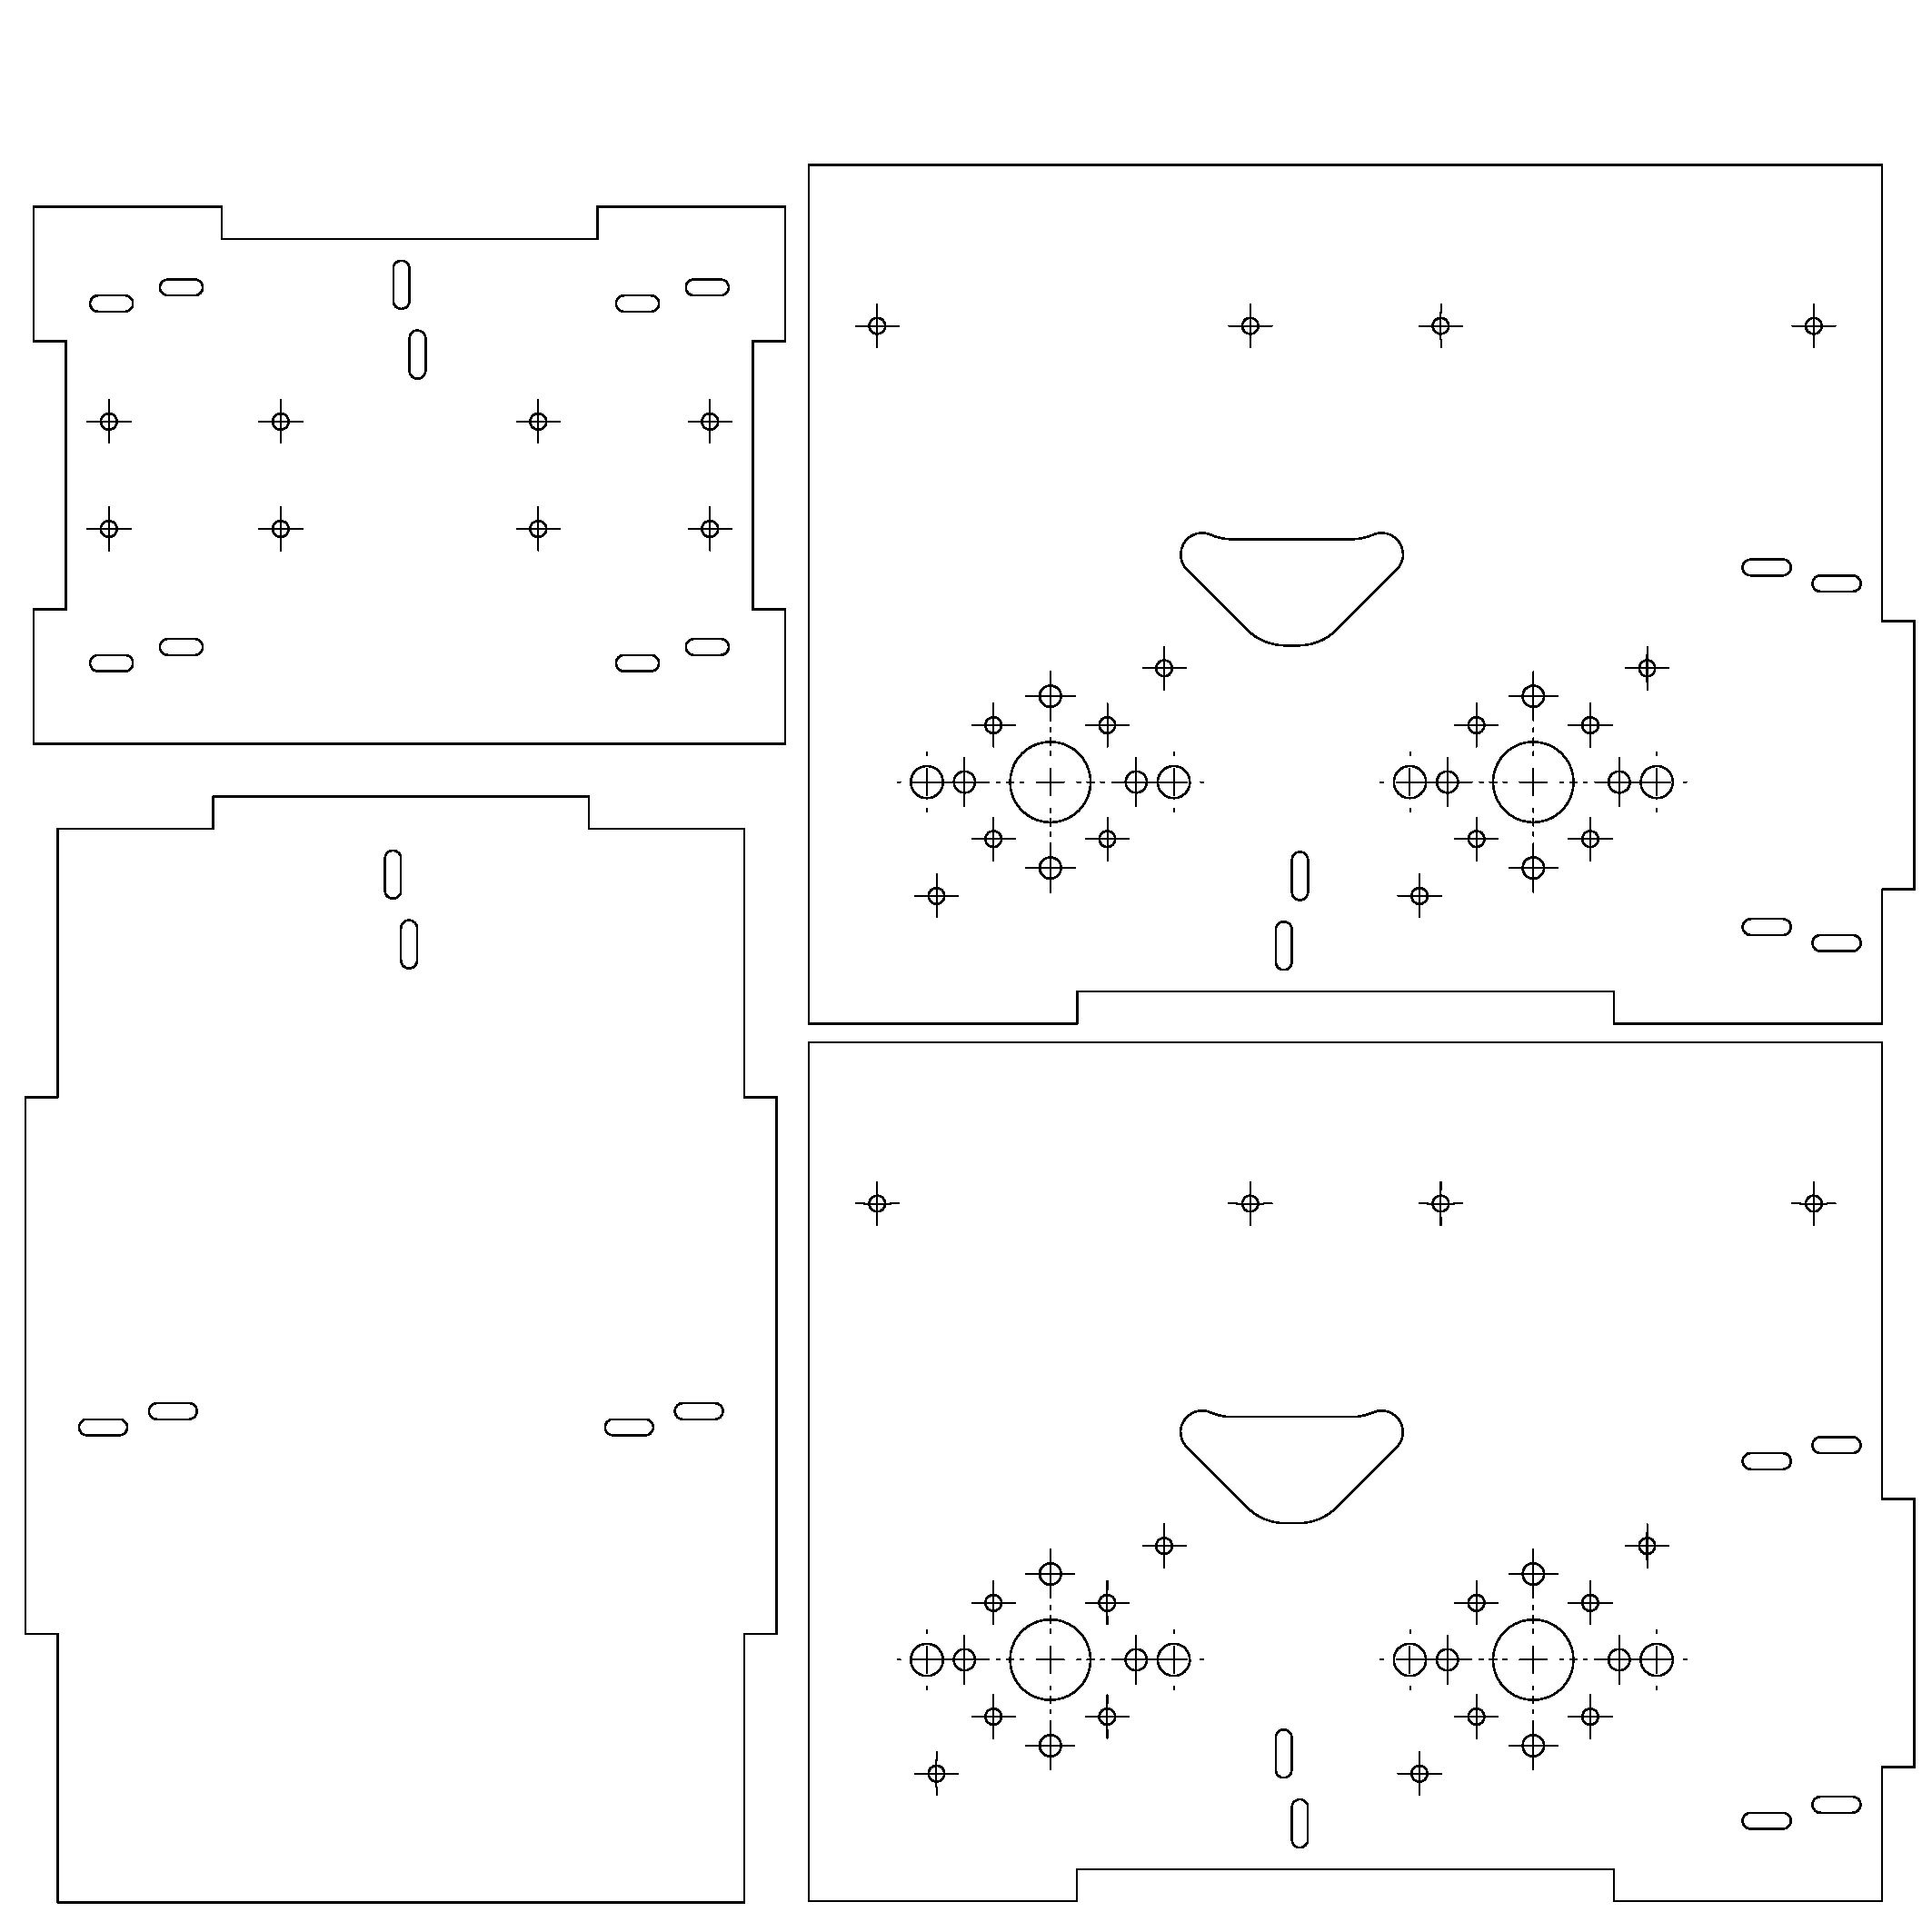
\includegraphics[clip, trim =0cm 0cm 0cm 0cm, page =1, width=0.4\textwidth]{images/mechanical/hip-6mm-360x360}
\caption{Original 'hip' design by Ben Bingham, 2016.}
\label{fig:original-hip}
\end{figure}

\subsection{Leg Guide}
The guiding system consisted of two parallel steel rods with ball bearings mounted on the `hip'. The ball bearings were mounted using a 3D printed holder, with one for each circular  bearing. 

\subsection{Limitations}

The leg mounting plate went through three design iterations after the original `hip' design before the final design was created, as seen in \cref{fig:CAD mounting plate final design}.

The original `hip' design had the following mechanical design flaws:

\begin{enumerate}
\item The 6 mm perspex box construction with on-board microncontroller and motor drivers was too heavy for efficient jumping action when compared to similar designs like \cite{Duperret} (1.3 kg), \cite{Kalouche2016} (2.5 kg), \cite{Wang2012} (4.2 kg) where there is a high leg torque to mass ratio.
\item The ball bearings are particularly heavy.
\item The mounting of the leg guide places a significant torque in all three cartesian coordinates being off-center from the center of mass.
\item The design of the leg guide requires the two steel rods to be perfectly parallel to remove resistance to movement, which is difficult to achieve practically.
\end{enumerate}

These problems were accounted for by replacing the original `hip' with a rigid aluminium mounting plate with off-board microcontroller and motor drivers. The leg guide consisting of parallel steel rods and ball bearings was replaced with a linear guide as seen in \cref{fig:drylin-linear-guide}.  

\begin{figure}
\centering
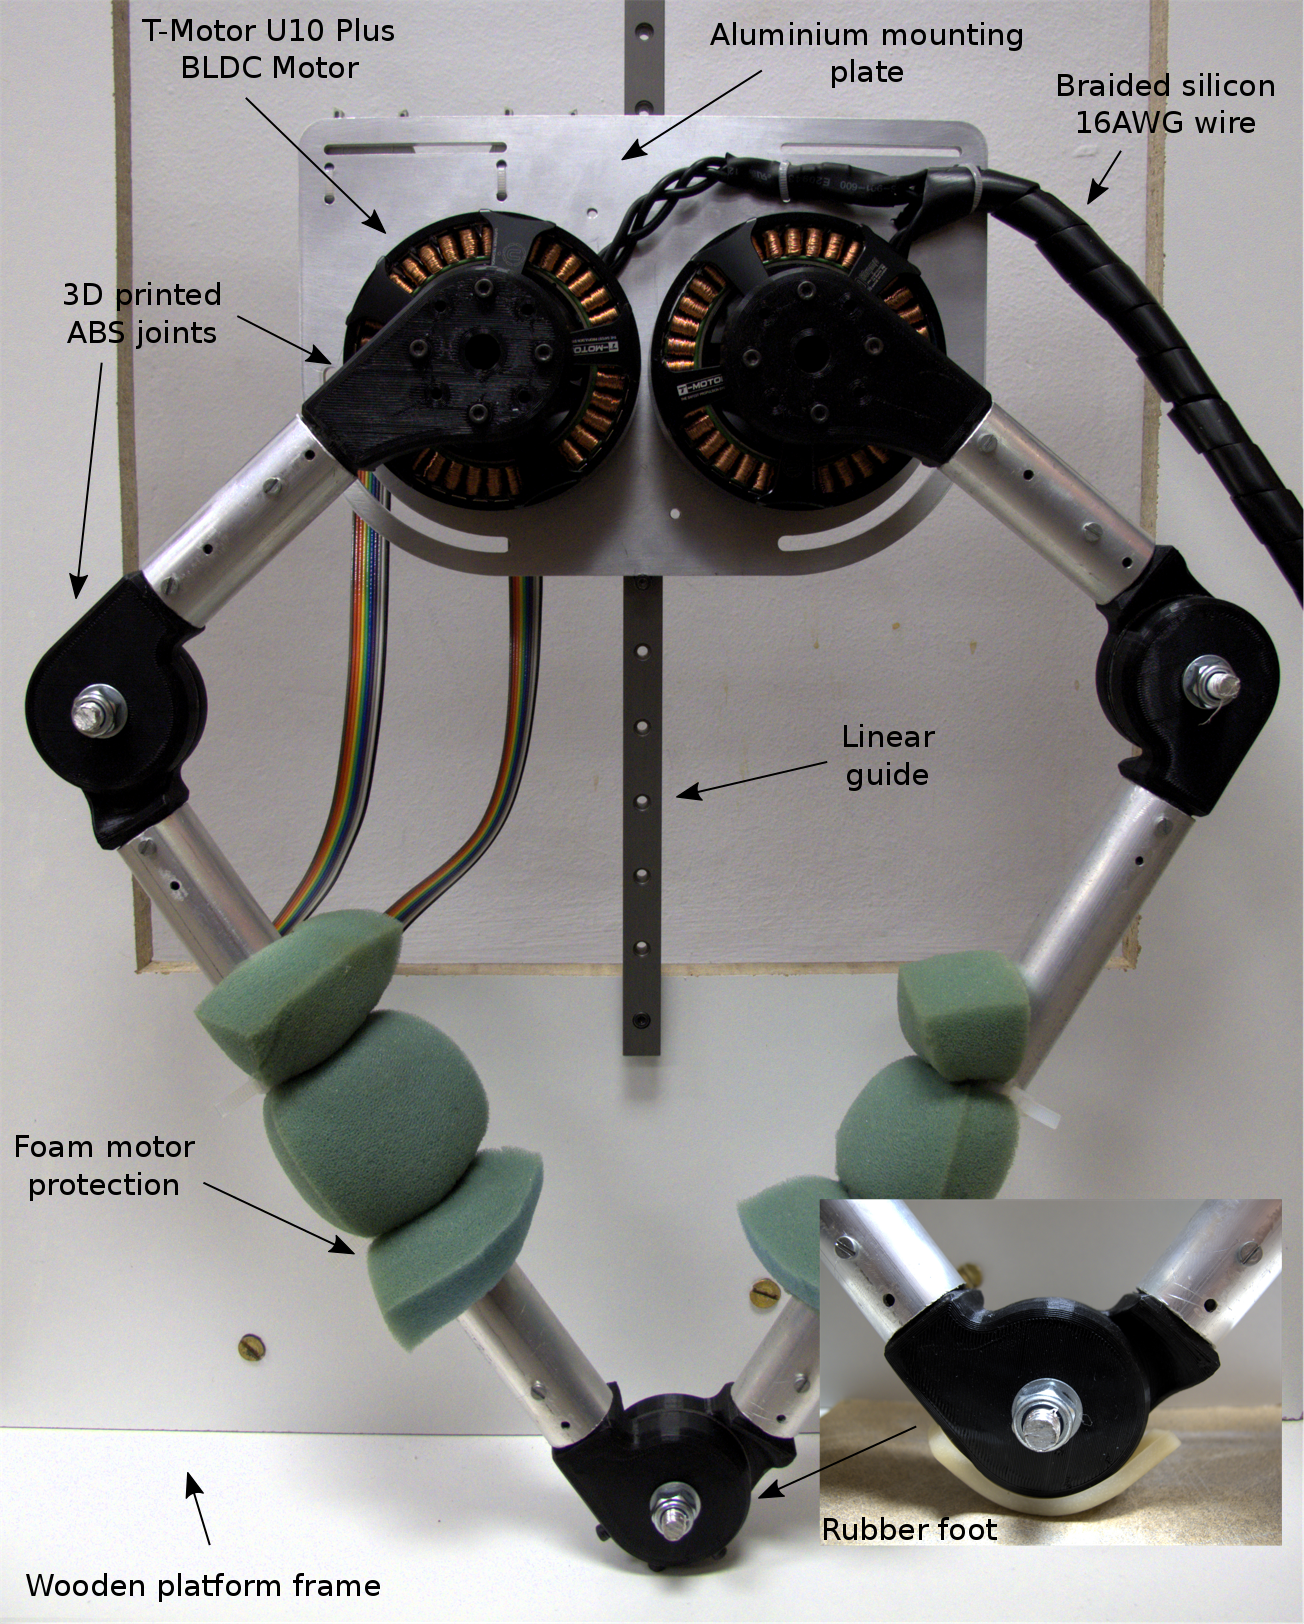
\includegraphics[width=0.8\textwidth]{images/mechanical/leg-mount-annotated} 
\caption{Final leg design mounted to platform and linear guide: front.}
\label{fig:Final leg design - front}
\end{figure}

\begin{figure}
\centering
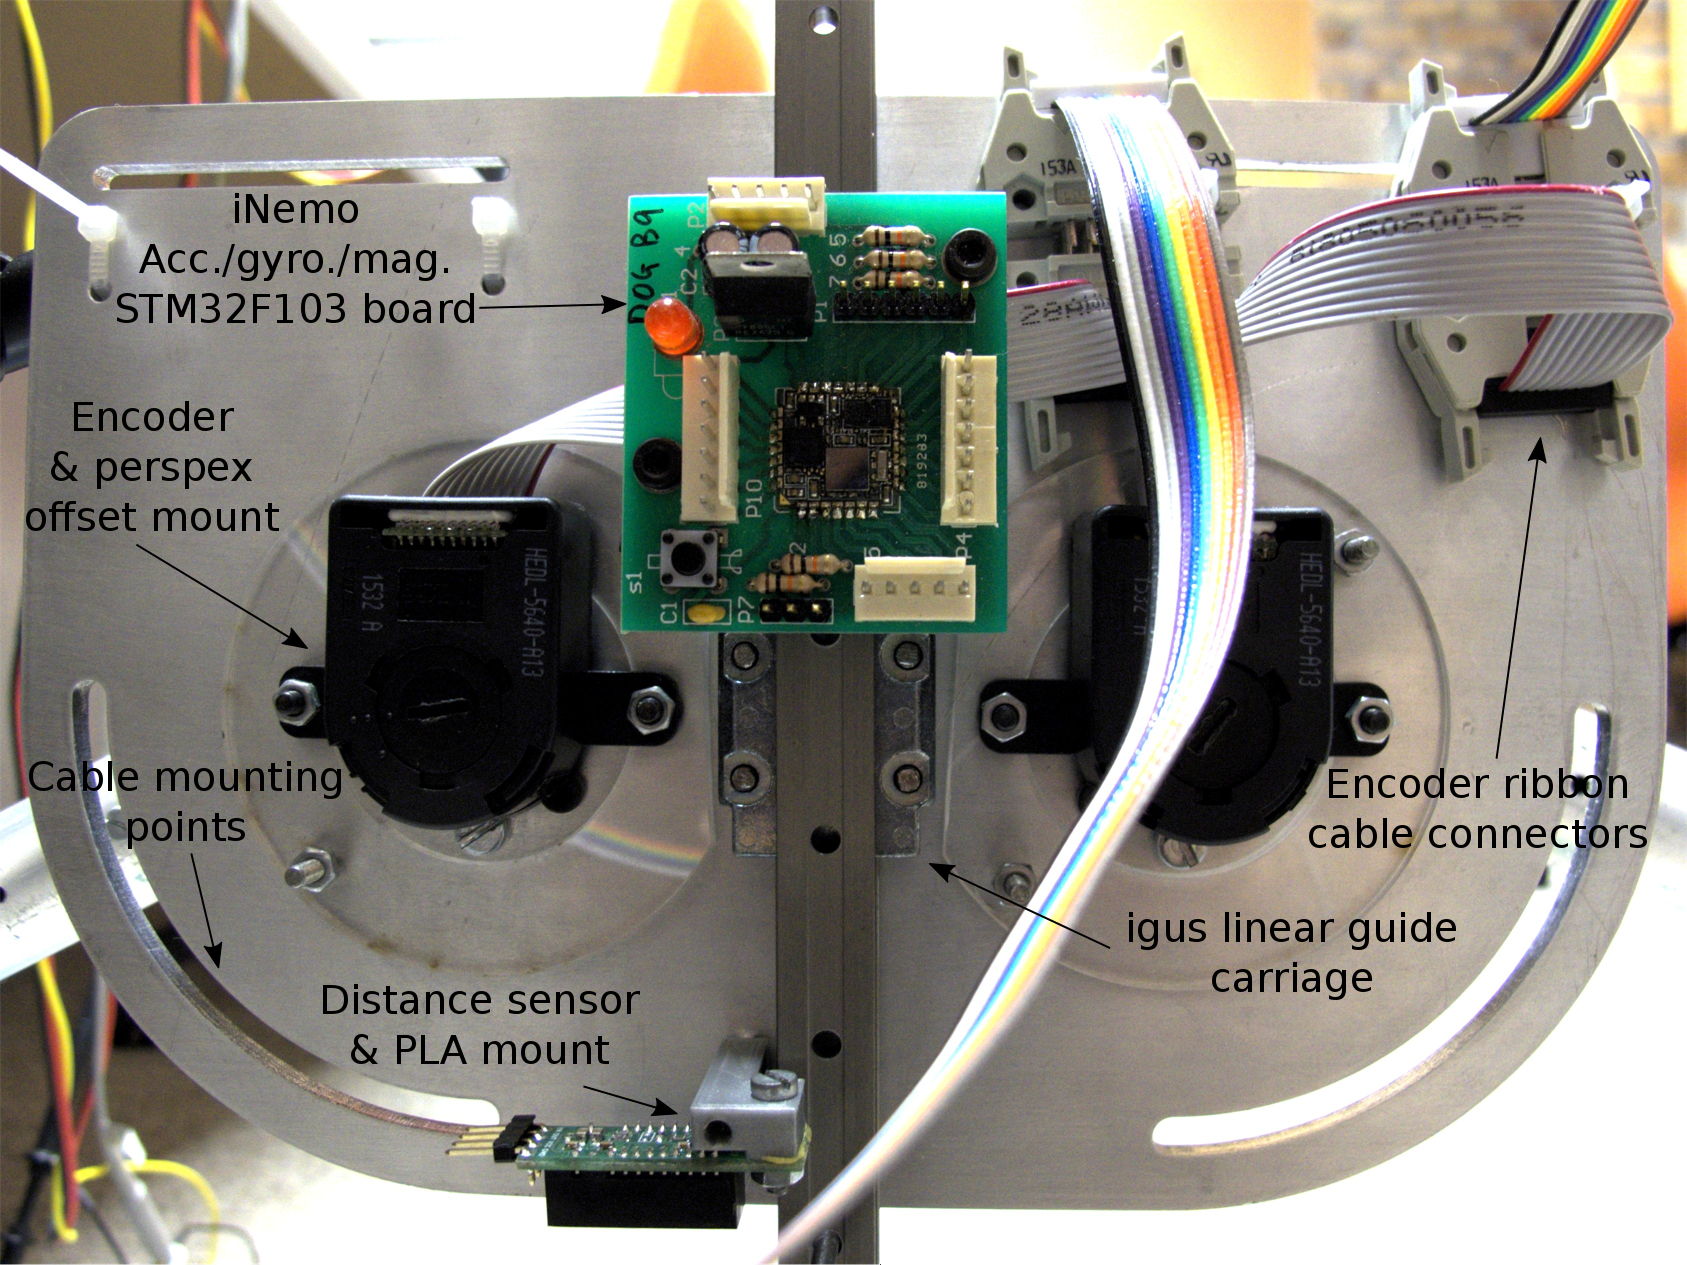
\includegraphics[width=0.8\textwidth]{images/mechanical/encoder-mount-annotated} 
\caption{Final leg design mounted to platform and linear guide: back.}
\label{fig:Final leg design - back}
\end{figure}

\section{Mechanics and Construction}

\subsection{Aluminium Mounting Plate Design}
\label{sec:Alumnium Mounting Plate Design}

The original mounting box described in \cref{sec:Original Leg Design} was replaced with a single mounting plate. 

In order to reduce the weight of the platform and to prevent damage to components during jump tests, the motor drivers and microcontroller were mounted off-board on a separate mounting plate - the final design of which can be seen in \cref{fig:Motor driver interface mounting plate}.

The plate that the motors and encoders mount to went through several iterations before the final design was used. A few major factors were considered in the design process, both for the motor mount and motor driver mount:
\begin{enumerate}
\item Perspex material was too flexible, especially considering the close tolerances of the motor mounts - aluminium was used instead of perspex as a more rigid material.
\item The motors when used in a high torque relatively static environment reach temperatures of close to $100^oC$ - this heat was noticeably better dissipated by aluminium.
\item The motor drivers perform better and are less likely to thermally cut-out if mounted on aluminium.
\item The center of mass of the robotic leg body was calculated and the linear guide mount was placed as close as possible to this point. This ensured as little torque as possible was placed on the linear guide which would lead to frictional losses and ware.
\item The iNemo accelerometer, gyroscope, magnetometer combination was placed as close as possible to the center of mass to ensure proper readings were achieved which accurately represented the robot dynamics.
\item Excess weight was cut wherever possible, most noticeably so above the motor mounting points.
\end{enumerate}


\begin{figure}
\centering
\subfloat[][CAD mounting plate V1.]{
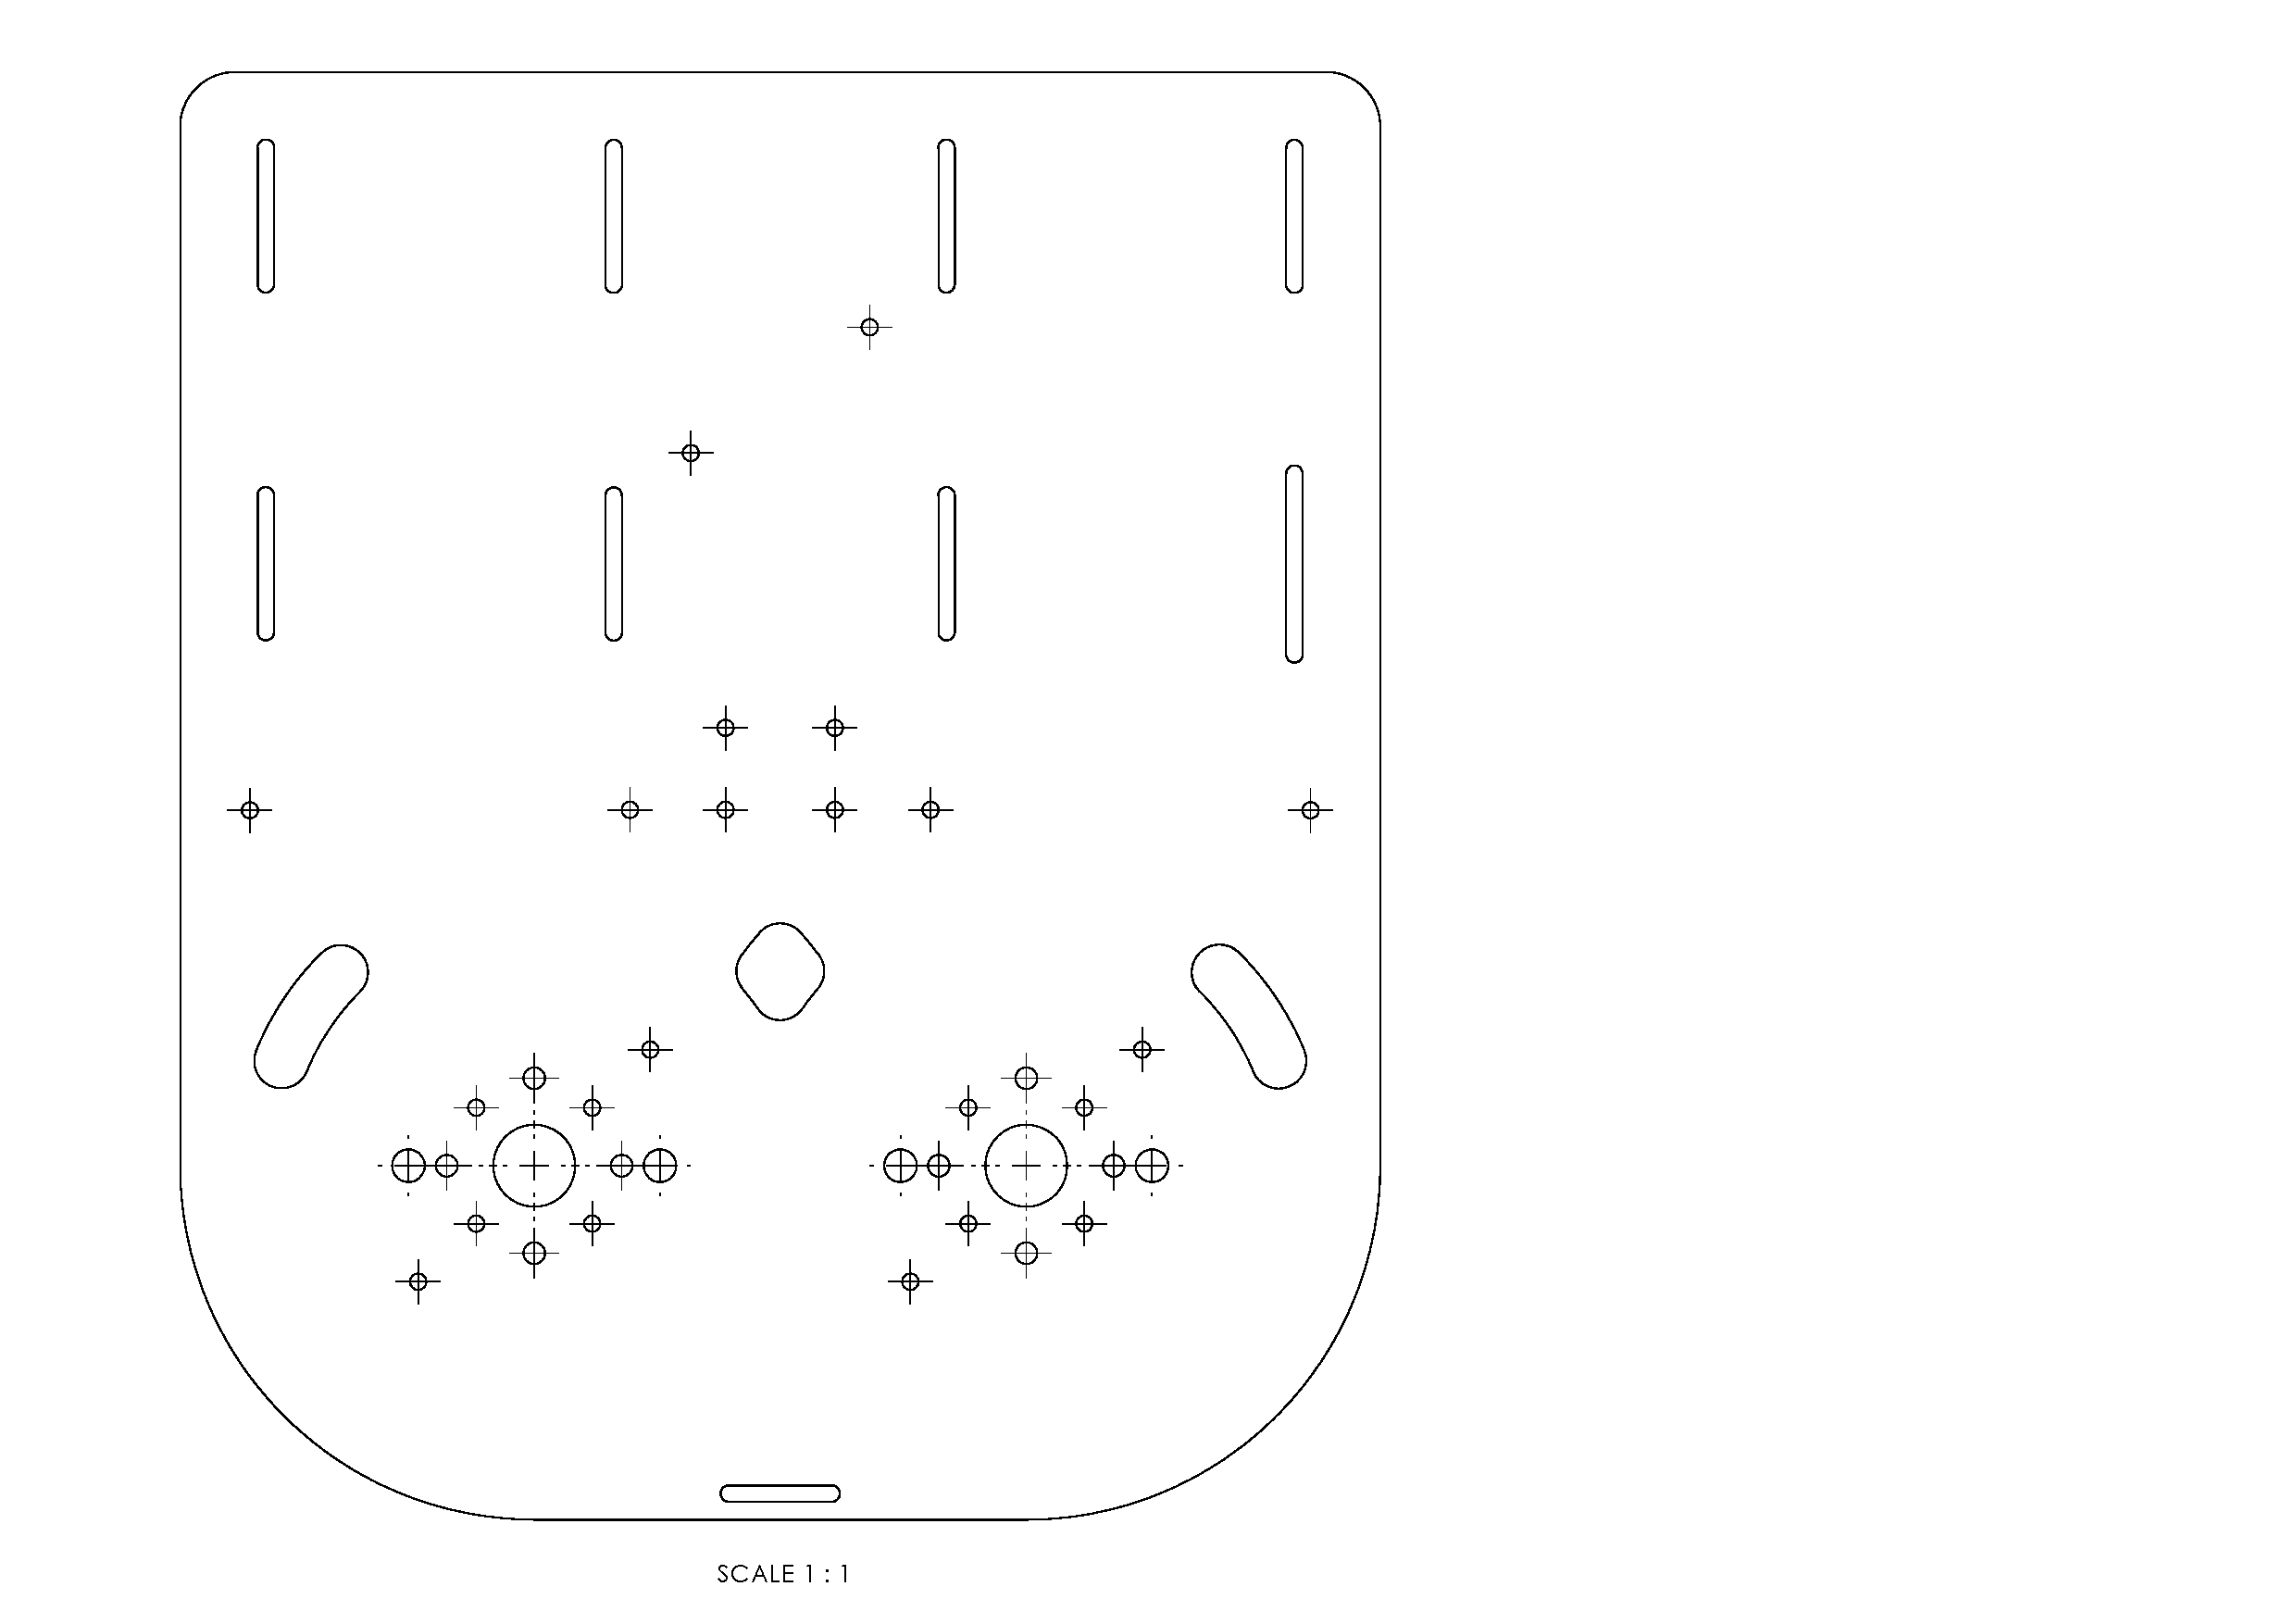
\includegraphics[clip, trim=2cm 0cm 16cm 1cm, page = 1, width=0.3\textwidth]{images/mechanical/laser-test-print-V1} 
\label{fig:CAD mounting plate V1}
}
\subfloat[][CAD mounting plate V3.1.3.]{
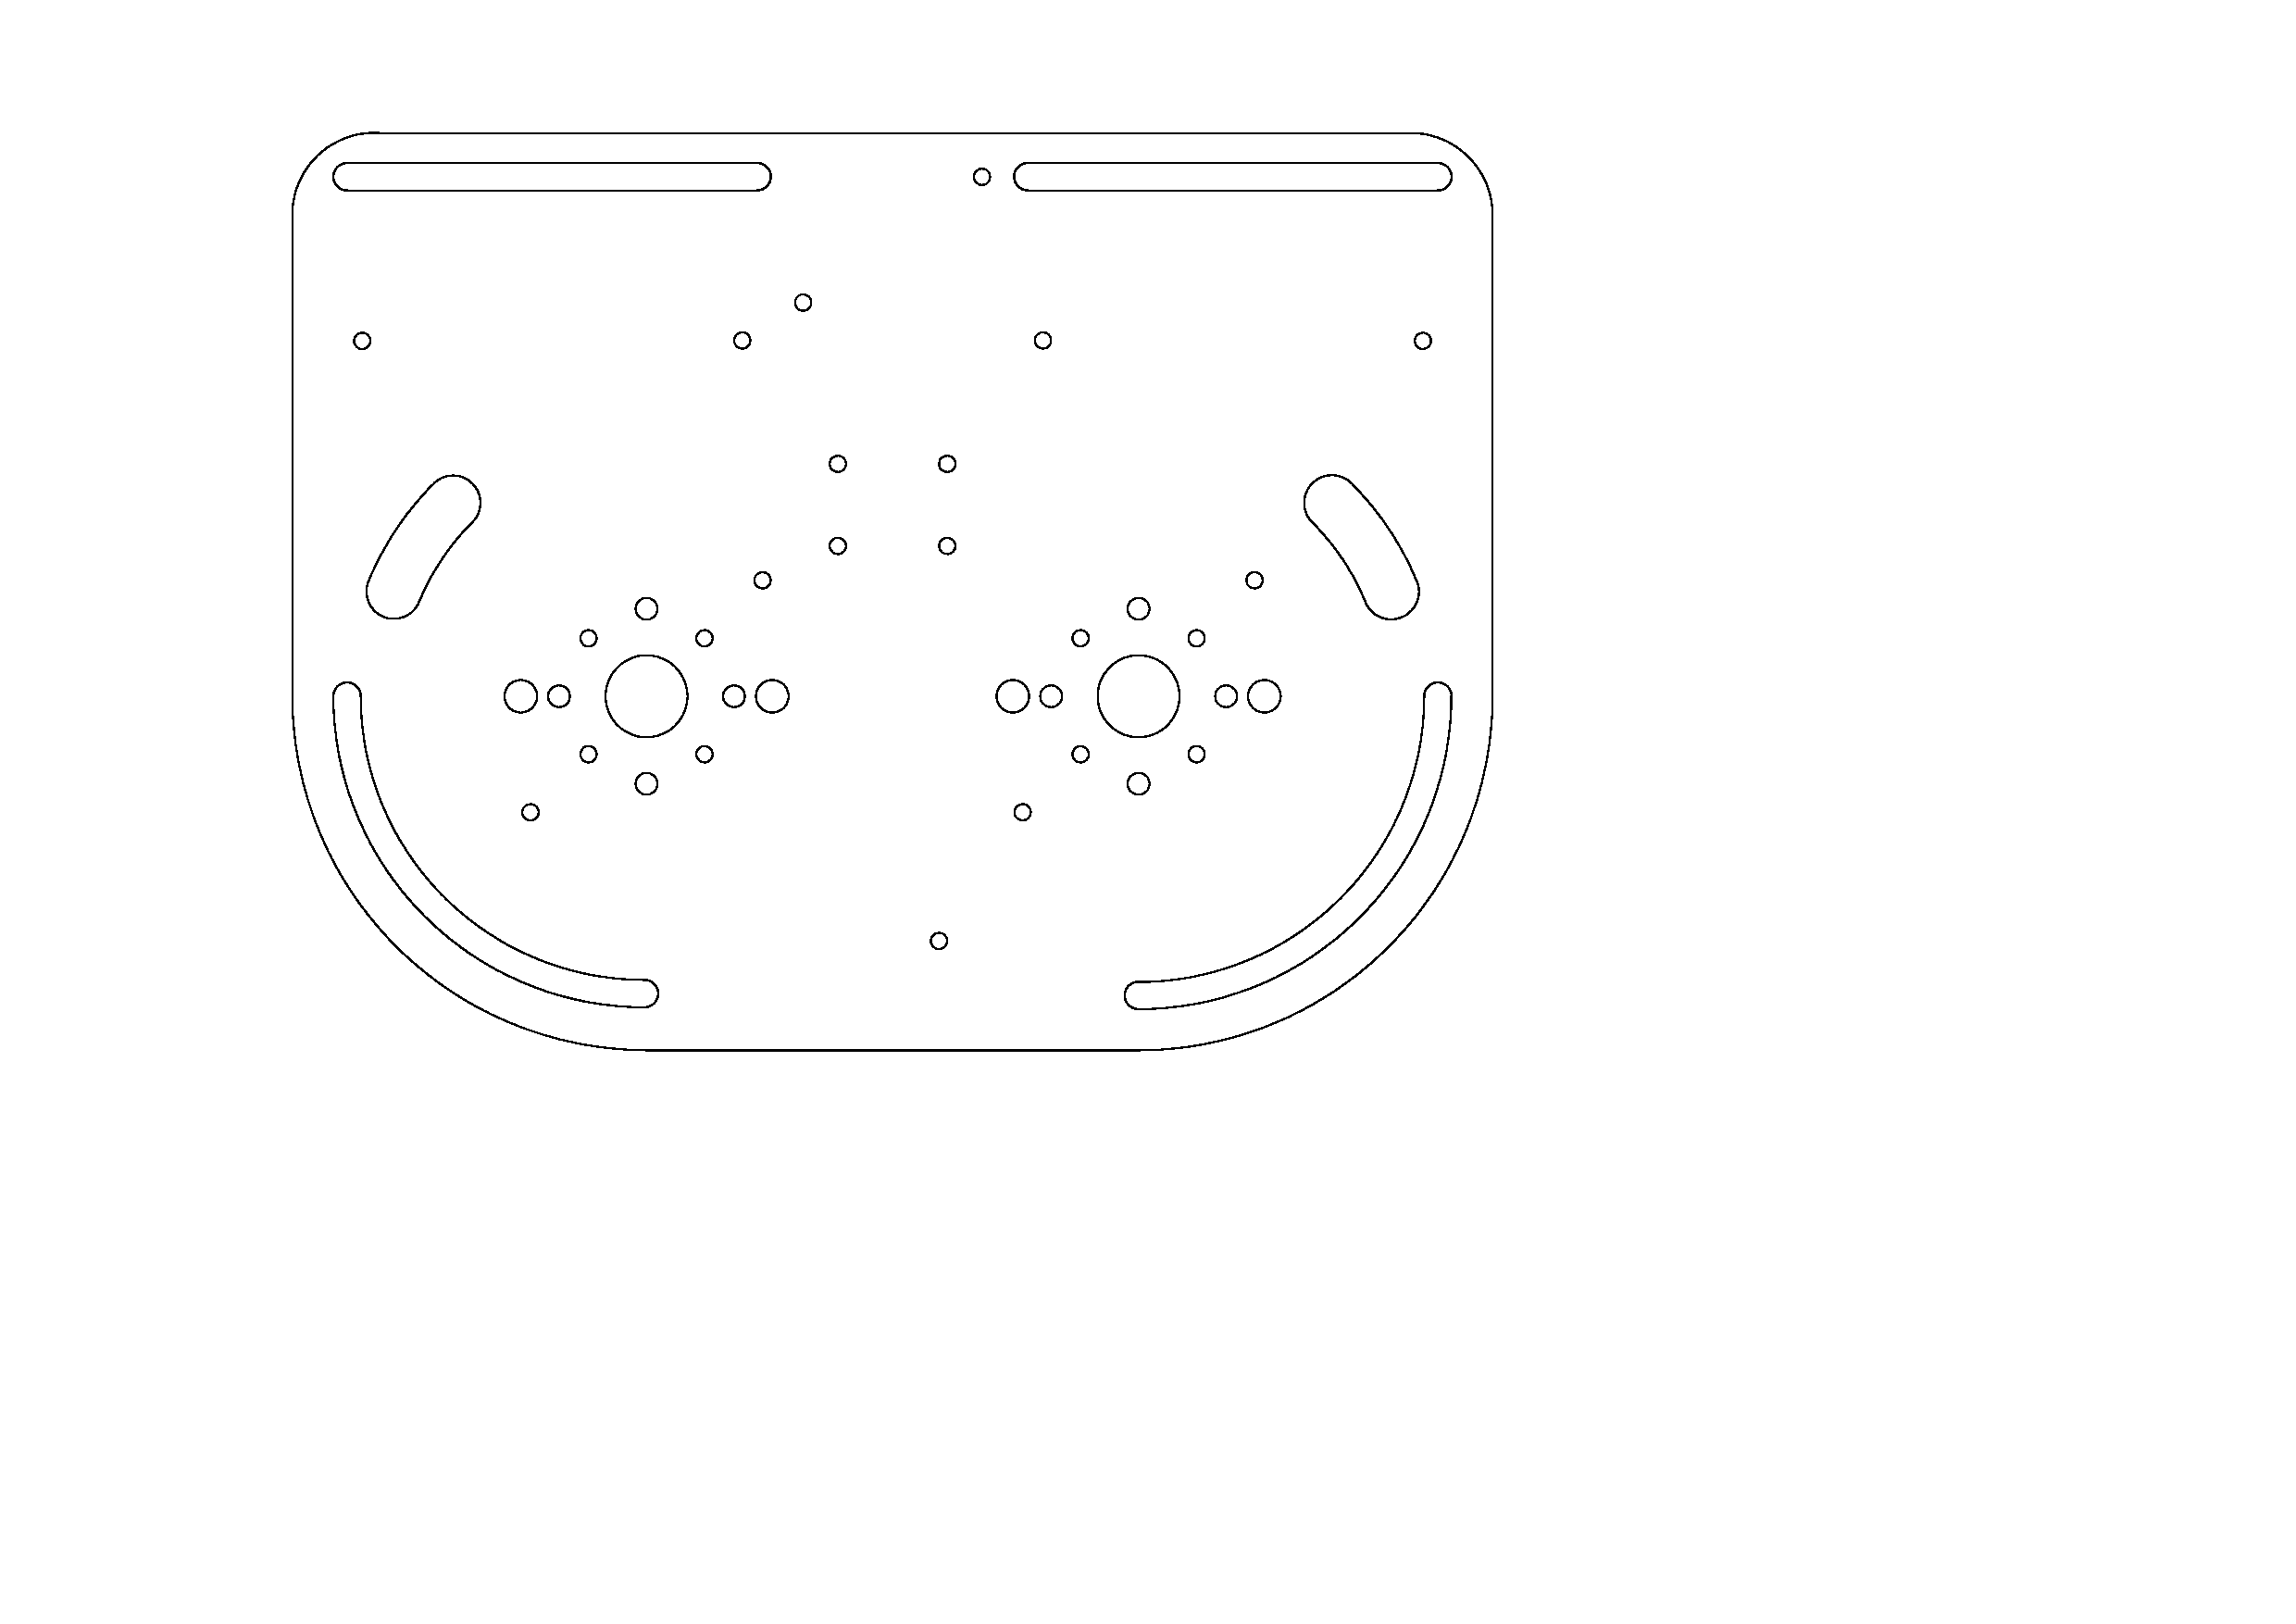
\includegraphics[clip, trim=5cm 10cm 14cm 2cm, page = 1, width=0.3\textwidth]{images/mechanical/laser-test-print-V313} 
\label{fig:CAD mounting plate V3.1.3}
}

\subfloat[][CAD mounting plate final design.]{
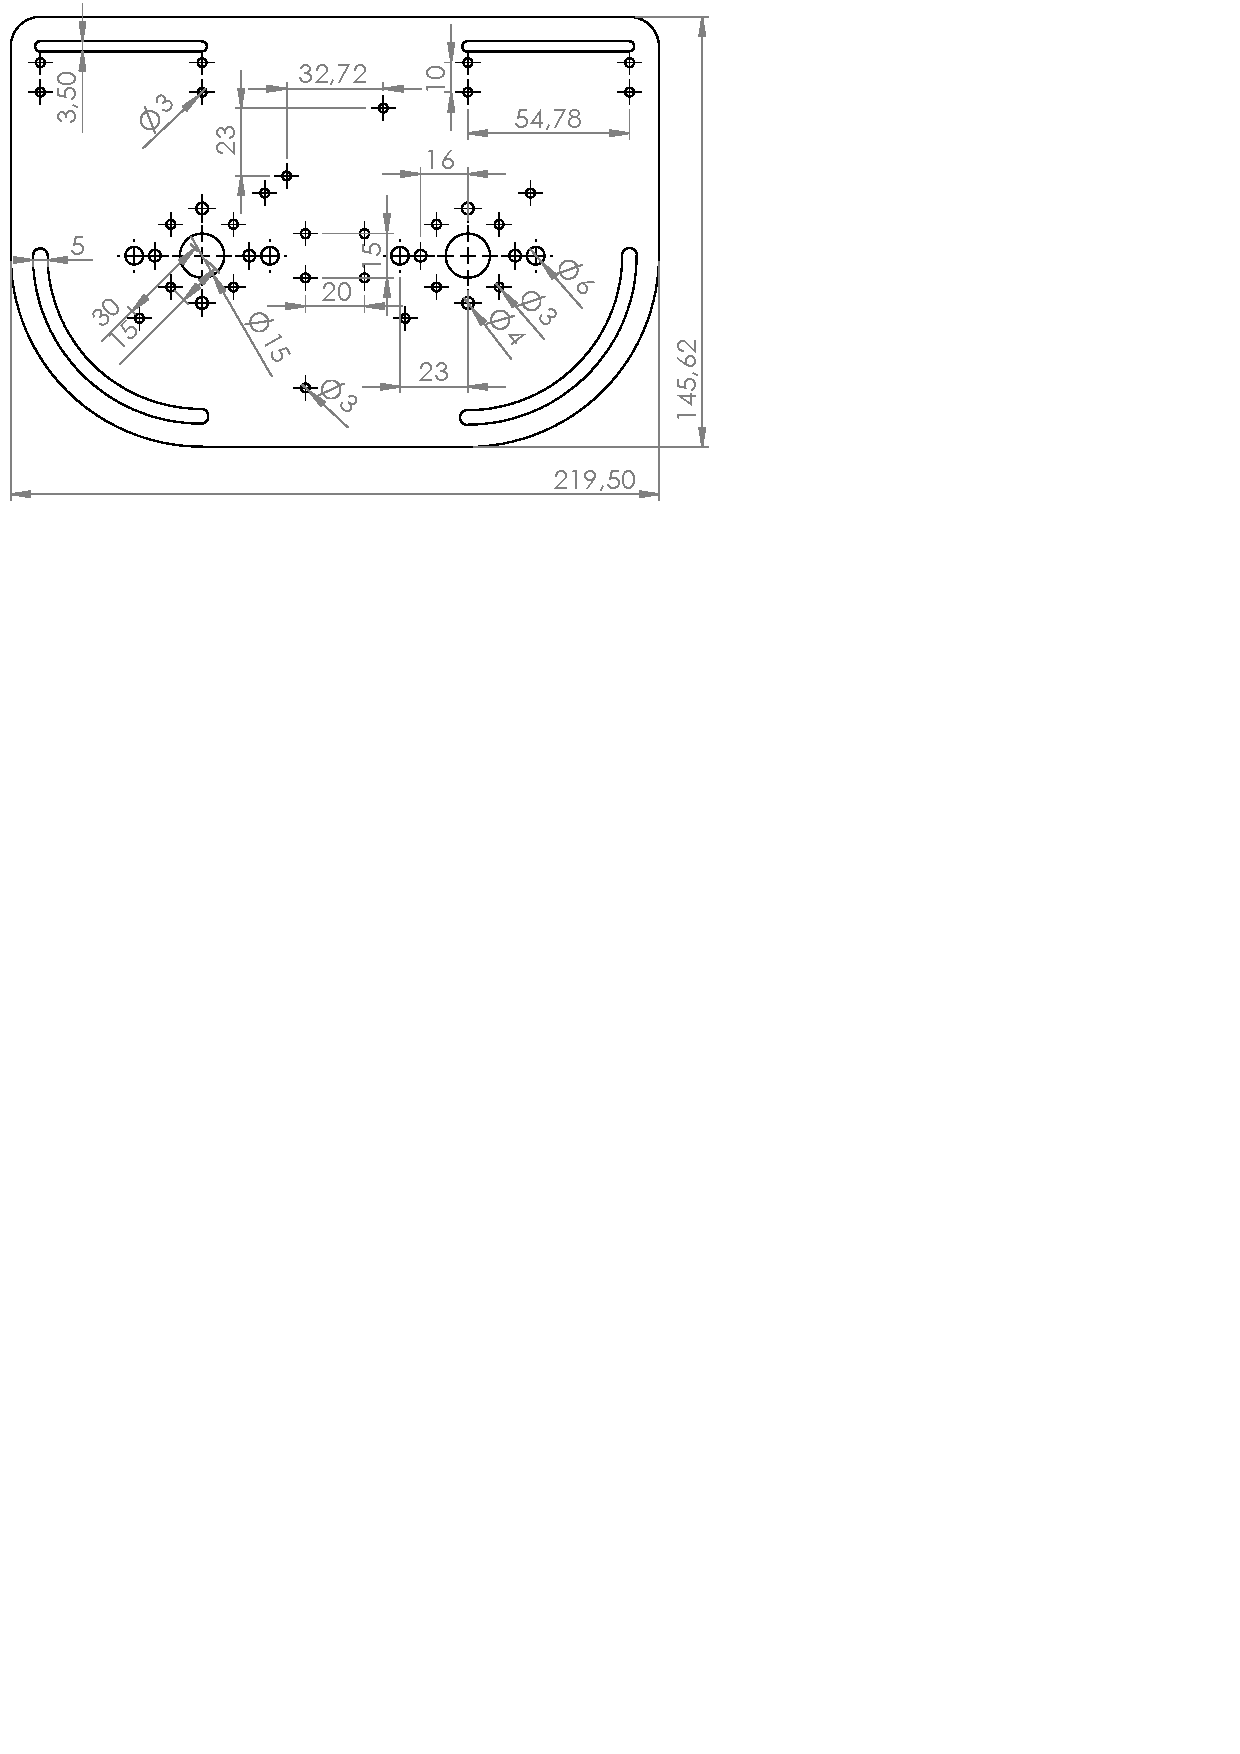
\includegraphics[clip, trim=0cm 21cm 9cm 0cm, page = 1, width=0.6\textwidth]{images/mechanical/main-plate-final} 
\label{fig:CAD mounting plate final design}
}
\caption{Leg mounting plate iterations.}
\label{fig:Leg mounting plate iterations}
\end{figure}

\begin{figure}
\centering
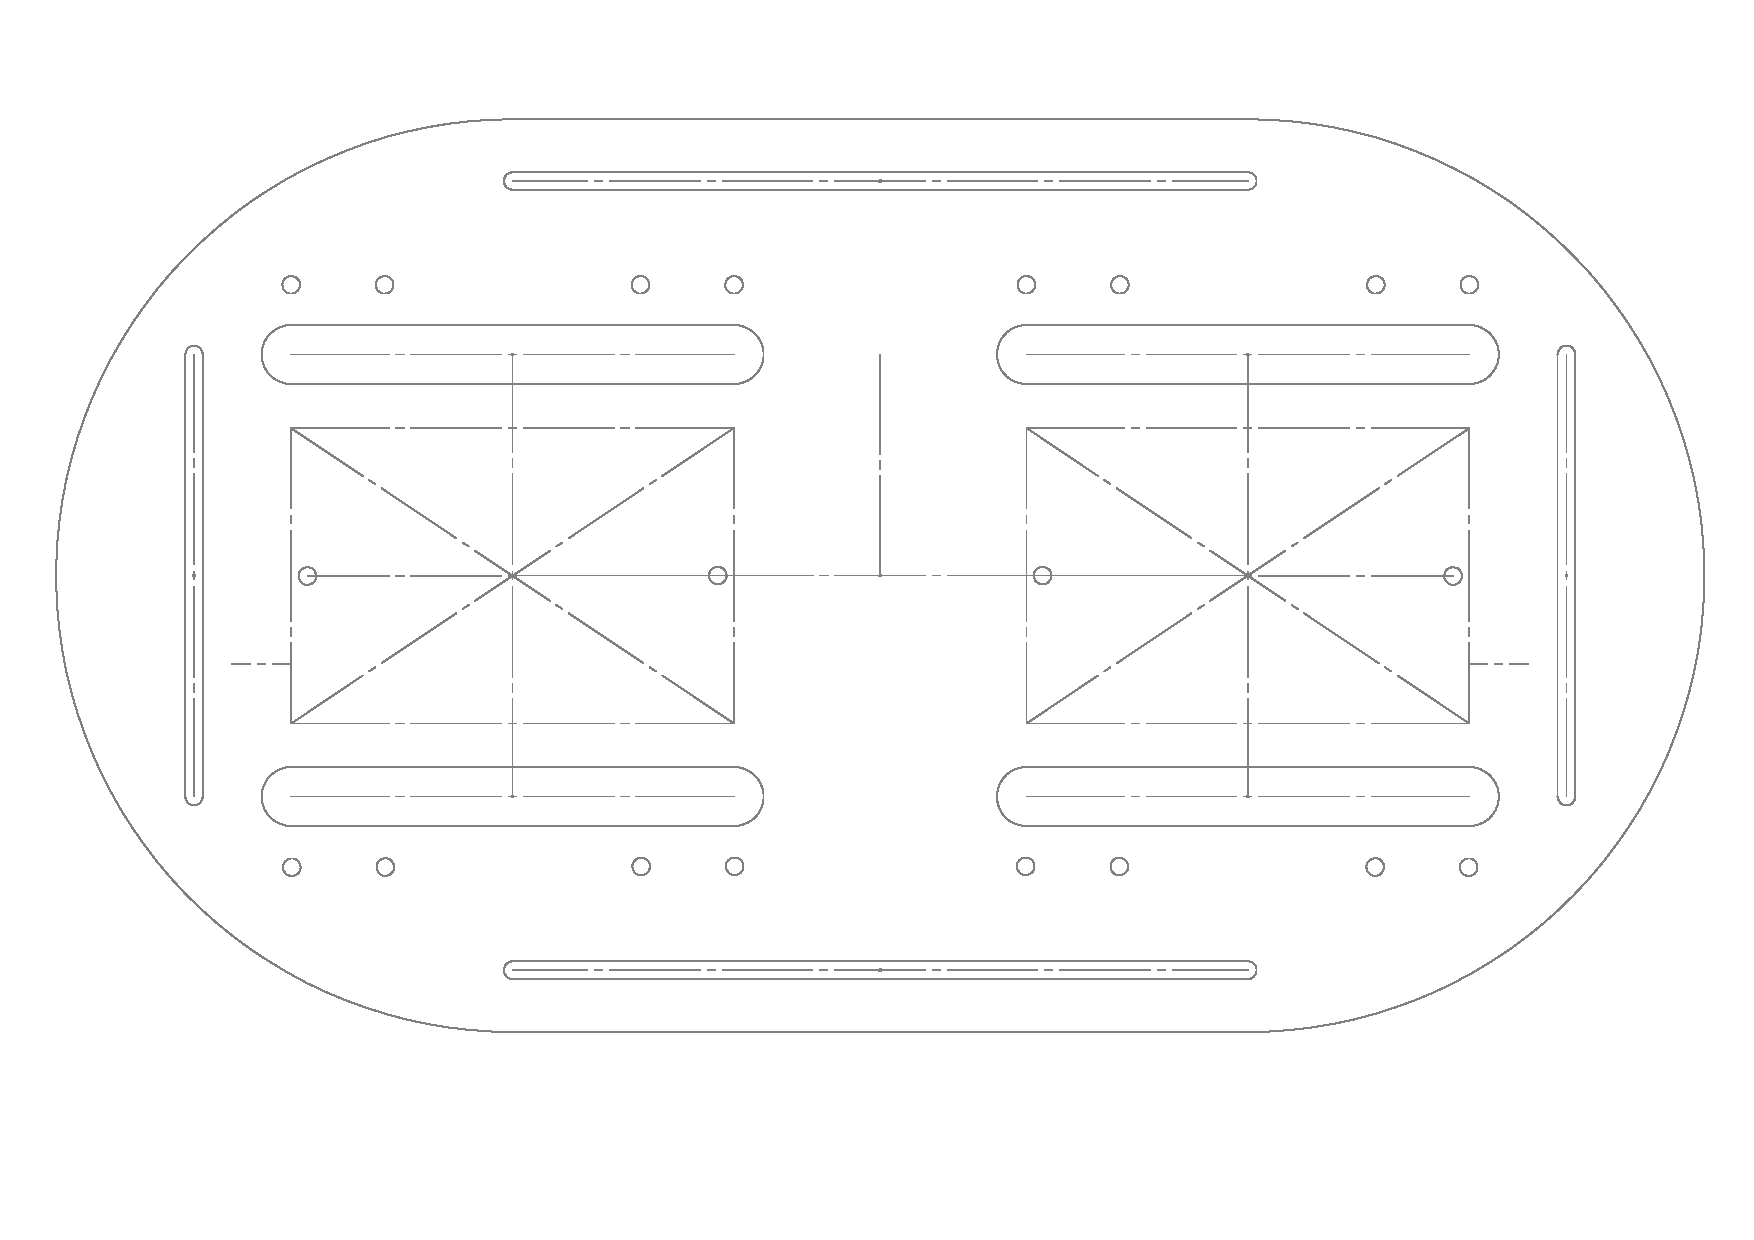
\includegraphics[width=0.6\textwidth]{images/mechanical/driver-mount-plate.pdf} 
\caption{Motor driver interface mounting plate.}
\label{fig:Motor driver interface mounting plate}
\end{figure}

\subsection{Leg Linkage and Foot Design}

The 4-bar linkage design of the leg was originally constructed by Ben Bingham in 2016 for completion of his undergraduate engineering vacation work in the mechatronics lab. The leg was constructed as follows:

\begin{itemize}
\item Three sets of rotational joints make up the linkage system. The joints were 3D printed using ABS plastic and used 3 mm screws to connect to the aluminium leg sections.
\item 8 mm loctite nut, bolt and washer combinations connected the joint components with perspex discs to reduce friction between the joints.
\item The aluminium leg sections were constructed of 25 mm diameter tubing to form a leg of 0.15 m and 0.3 m sections including the joints. 
\end{itemize}

The leg had a number of design flaws that will be improved upon in the implementation of the Mechatronics Lab Cheetah project with the leg being redesigned by Callen Fisher. These issues are listed below:

\begin{enumerate}
\item The joints provide significant friction when under torque outside of the two degrees of freedom of the leg. 
\item The resistance to movement provided by the joints in normal operation is directly related to the amount of torque tightening on the nut and bolt. 
\item The nuts and bolts slowly work themselves loose under normal operation due to vibrations and impact.
\item The motor joints, being off-set from the motor shafts, place significant torque on the motor shafts under impact.
\end{enumerate} 

Without the proper material to provide friction during foot placement on the ground, lateral slipping occurs as seen in \cref{fig:foot-slipping}. To improve the grip of the foot, the following design choices were made:

\begin{enumerate}
\item 80 to 120 grit sandpaper was placed on the platform to emulate the material encountered by a Cheetah in normal operation, namely dirt and gravel.
\item A rubber mould was made, by mixing and setting rubber components, before being attached to the foot using 3 mm hex screws.
\end{enumerate}

The combination of sandpaper and rubber foot stopped lateral slipping from occurring.

\begin{figure}
\centering
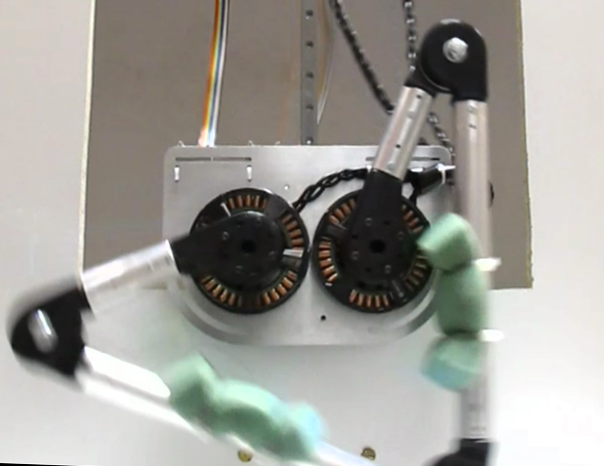
\includegraphics[width=0.6\textwidth]{images/experiments/lateral-slipping} 
\caption{Leg foot lateral slipping.}
\label{fig:foot-slipping}
\end{figure}

\subsection{Testing Platform}
\label{subsec:Testing Platform}

The testing platform was designed to be limited to a vertical axis of movement. This allows robust testing of the hopping capabilities of Baleka. In future experimentation a rotational hinged platform can be used to test forward hopping trajectories. 

The original platform design used two parallel $16\ mm$ tool steel rods with ball bearings attached to the leg platform. This not only added extra weight, but also made it difficult to properly mount the rods parallel to avoid friction. 

The original setup was replaced with an igus linear guide as seen in \cref{fig:drylin-linear-guide}, specifically the TW-04-12 DryLin T miniature slide carriage along with the appropriate rail.

A rail of $0.6\ m$ was used which resulted in a potential hopping height of $0.4\ m$. This height proved to be adequate given the motor driver's $60\ A$ current limit which in practise resulted in a maximum hopping height of just under $0.4\ m$. Further hopping experiments performed with the linear guide platform can be seen in \cref{chap:Experimental Testing}.

The linear guide rail was mounted on a wooden frame with a heavy $3\ kg$ wooden counterweight on the base. The choice of wood for the frame was to reduce vibrations and for ease of construction. The heavy wooden base ensured the platform was stable during jump experimentation.

Despite specifications of the rail not requiring lubrication, a basic oil based lubricant was used and significantly reduced friction caused by forward rotational torque of the carriage on the linear guide rail.

To simulate the environment and platform used in the hopping experiments a CAD assembly was generated, as seen in \cref{fig:Linear guide mounted leg model}, as well as a virtual world Matlab model. This allowed the leg to be manipulated and dropped on the platform to see how it would behave. The resulting tests ensured the testing platform would have a good chance of performing well in real life experiments. Given that the linear guide system was a significant capital investment this was necessary.

\begin{figure}
\centering
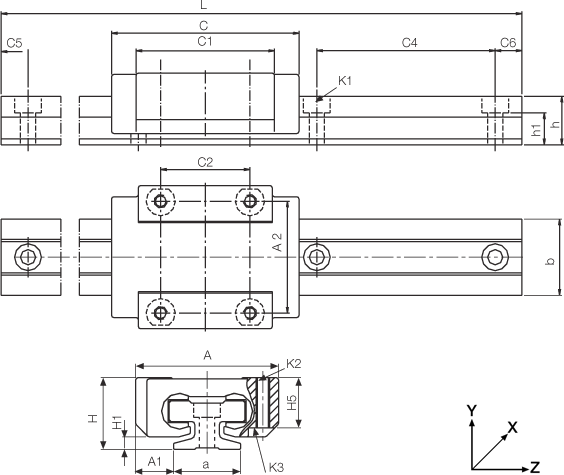
\includegraphics[width=0.6\textwidth]{images/mechanical/drylin-linear-guide.png} 
\caption{igus DryLin T - Low-profile linear guide.}
\label{fig:drylin-linear-guide}
\end{figure}


\begin{figure}
\centering
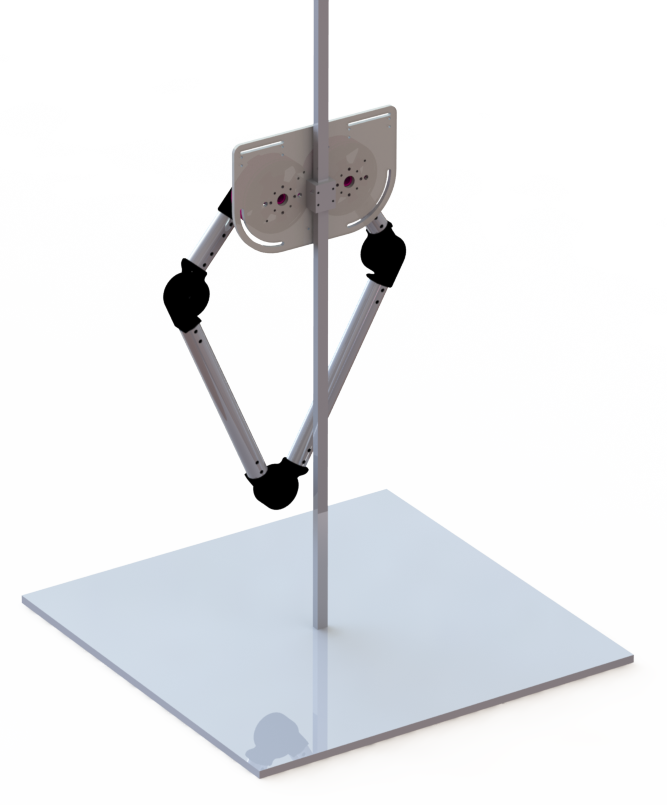
\includegraphics[width=0.4\textwidth]{images/mechanical/back-shot.png} 
\caption{Linear guide mounted leg model (CAD Solidworks assembly).}
\label{fig:Linear guide mounted leg model}
\end{figure}

\section{Mass Distribution}

The calculation of the mass and center of mass (COM) was critical for making the following design choices:

\begin{itemize}
\item Placement of the iNemo sensor board as close to the COM as physically possible (seen in \cref{fig:Final leg design - back}).
\item Mounting of the linear guide carriage as close to the COM to minimize torque and stress placed on guide rail during jumping, as well as interference to jump dynamics (seen in \cref{fig:Final leg design - back}).
\item Calculation of jump dynamics as in \cref{chap:Dynamic Modelling}.
\end{itemize}

The mass of individual leg components was first calculated manually using a scale, the log of which can be seen in \cref{tbl:Leg component mass}. The total mass of $2.2\ kg$ from this log was used in all dynamics, modelling and simulation calculations. 

The iNemo and linear guide carriage are of minimal mass and were not included in the manual mass calculation.

The center of mass was simulated in Solidworks. The material properties of each component were first configured appropriately. 

For simulation the leg radial set-point was set to $0.3\ m$ - this is the value of the leg radius during flight, freefall, impact, and compliant landing phases of jumping as seen in \cref{sec:Jump Test}. This ensures the COM calculation is accurate for the majority of the jump. 

In reality the center of mass (COM) moves negligibly with the foot position. The reason for this can be seen in \cref{fig:Mass distribution of leg assembly} where the mass distribution simulation shows the majority of the mass is concentrated around the COM, in red. The colour legend in \cref{tbl:Solidworks leg assembly mass distribution} explains the colour code and shows the simulated mass of each component.

In \cref{fig:Mass distribution of leg assembly} the COM is clearly shown as a black and white checker board circle with the distance from critical points shown on the second figure. The linear guide carriage is mounted just above this point along with the iNemo mounted with spacers above the carriage - it was not possible, due to the motor mounts, to place these components physically closer.

\subsection{Limitations}

The COM was only calculated in the two dimensional case. A significant torque was found to exist in the third dimension during experimentation that caused the leg to twist forward on the mount. This provided significant friction on the linear guide rail. In future designs the COM should be calculated in the third dimension and the motors possibly mounted coaxially on either side of the aluminium plate - this would have minimized the forward torque as the motors are the components with the most mass.

\begin{table}[]
\centering
\begin{tabular}{llll}
\textbf{Item}             & \textbf{Mass (g)} & \textbf{No.} & \textbf{Total Mass (g)} \\
T-Motor U10 Plus          & 500               & 2            & 1000                    \\
Servo drive               & 123.9             & 2            & 247.8                   \\
Servo drive mounting card & 50.7              & 2            & 101.4                   \\
Leg                       & 500               & 1            & 500                     \\
Plate                     & 350               & 1            & 350                     \\
\textbf{Total}            & \textbf{}         & \textbf{}    & \textbf{2199.2}        
\end{tabular}
\caption{Leg component mass.}
\label{tbl:Leg component mass}
\end{table}

% Please add the following required packages to your document preamble:
% \usepackage[table,xcdraw]{xcolor}
% If you use beamer only pass "xcolor=table" option, i.e. \documentclass[xcolor=table]{beamer}
\begin{table}[]
\centering
\begin{tabular}{llll}
\textbf{Colour legend}                          & \textbf{Component}    & \textbf{No.} & \textbf{Mass (g)} \\
\cellcolor[HTML]{FE0000}                        & T-Motor U10 Plus      & 2            & 424.56            \\
\cellcolor[HTML]{CB0000}                        & Mounting Plate        & 1            & 378.86            \\
\cellcolor[HTML]{010066}{\color[HTML]{000000} } & Linear Guide Carriage & 1            & 100.37            \\
\cellcolor[HTML]{3531FF}                        & ABS Motor Joint       & 2            & 50.55             \\
\cellcolor[HTML]{3531FF}                        & Long Linkage          & 2            & 46.40             \\
\cellcolor[HTML]{3531FF}                        & Joint                 & 5            & 39.83             \\
\cellcolor[HTML]{3531FF}                        & Foot Joint            & 1            & 39.63             \\
\cellcolor[HTML]{3531FF}                        & Short Linkage         & 2            & 12.81             \\
\cellcolor[HTML]{3531FF}                        & Washer Bearing        & 3            & 2.41              \\
\textbf{Total:}                                 & \textbf{}             & \textbf{}    & \textbf{1793.88} 
\end{tabular}
\caption{Solidworks leg assembly mass distribution.}
\label{tbl:Solidworks leg assembly mass distribution}
\end{table}

\begin{figure}
\centering
\subfloat[][Mass distribution simulation.]{
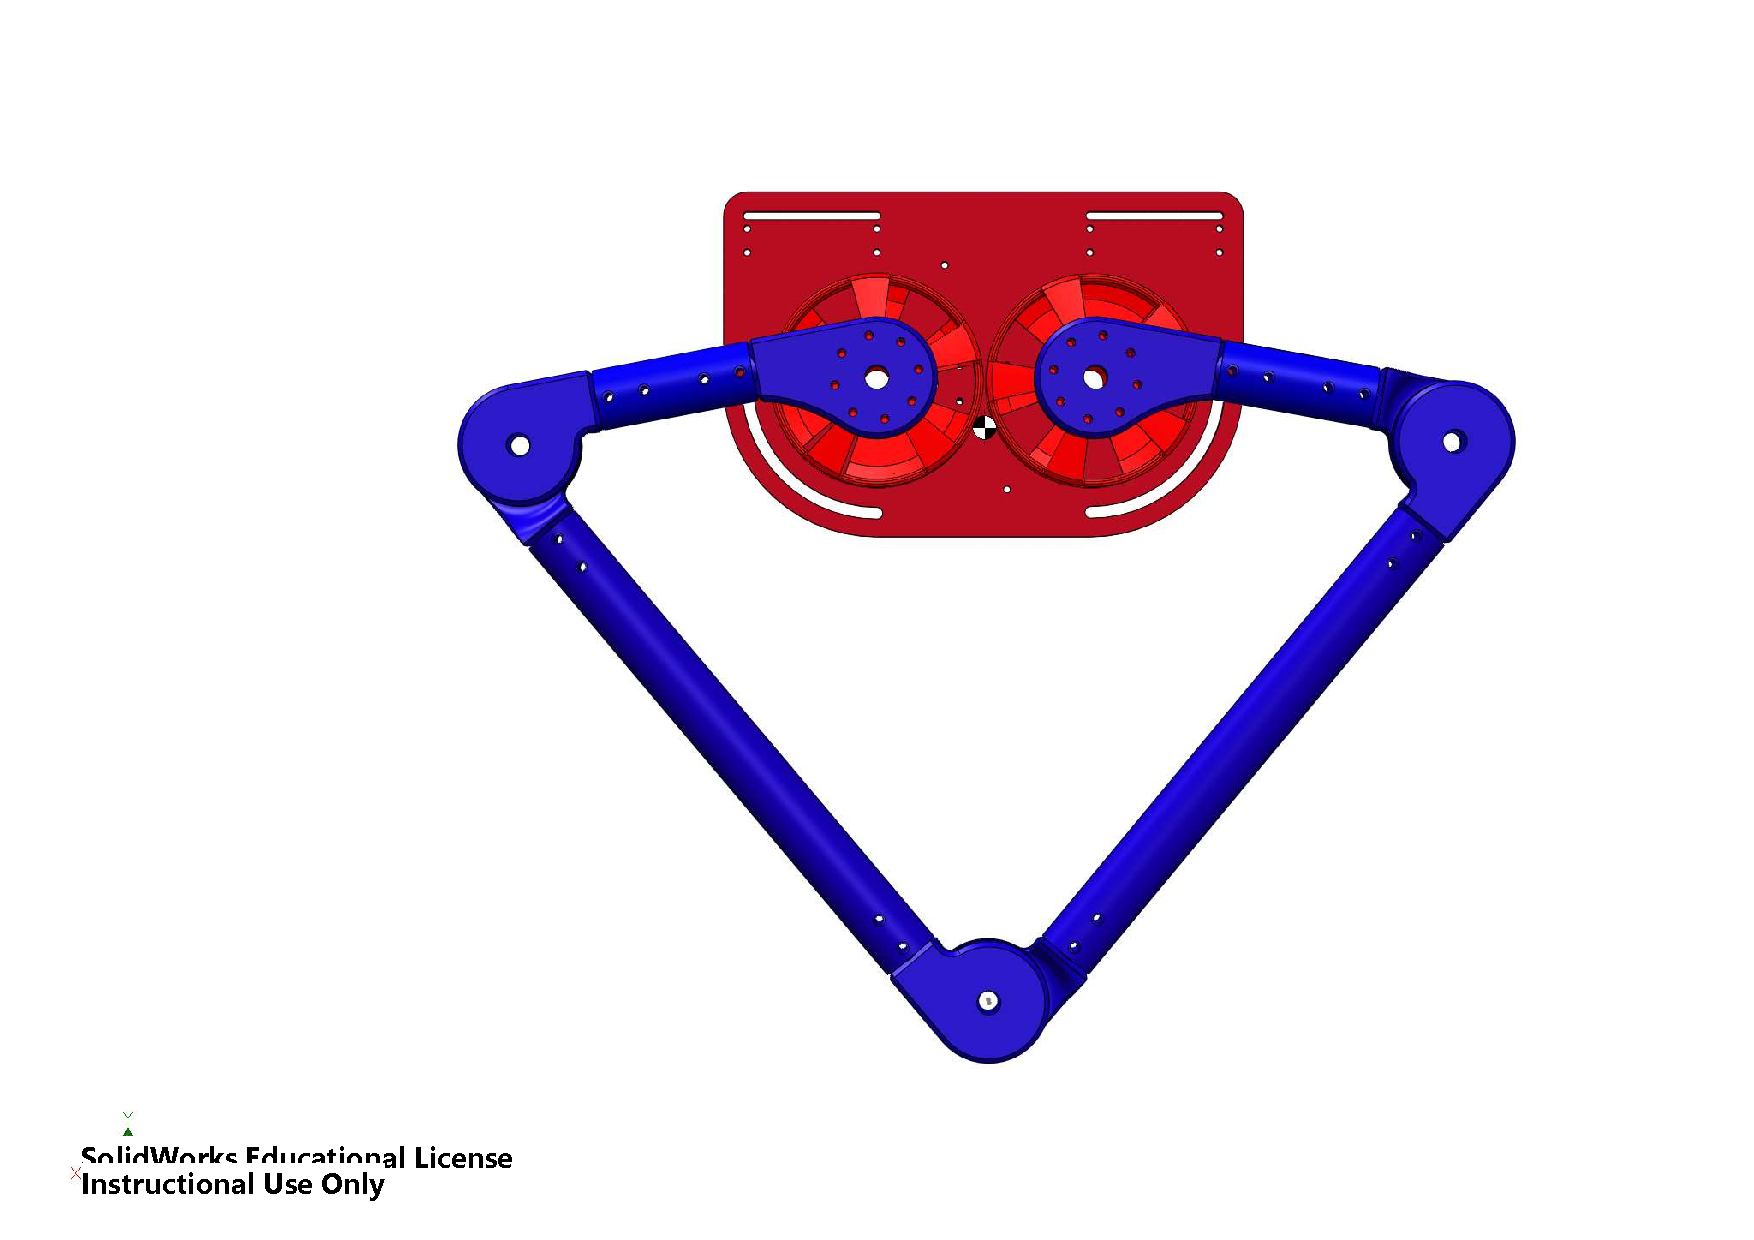
\includegraphics[clip, trim=5cm 2cm 4cm 2cm, page = 1, width=0.7\textwidth]{images/mechanical/assembly-com-distribution.pdf} 
}
%\subfloat[][Mass distribution colour legend (grams).]{
%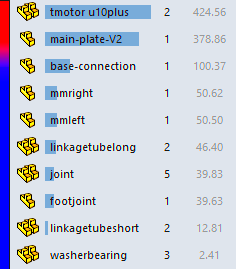
\includegraphics[width=0.3\textwidth]{images/mechanical/com-distribution} 
%}

\subfloat[][Center of mass of leg assembly.]{
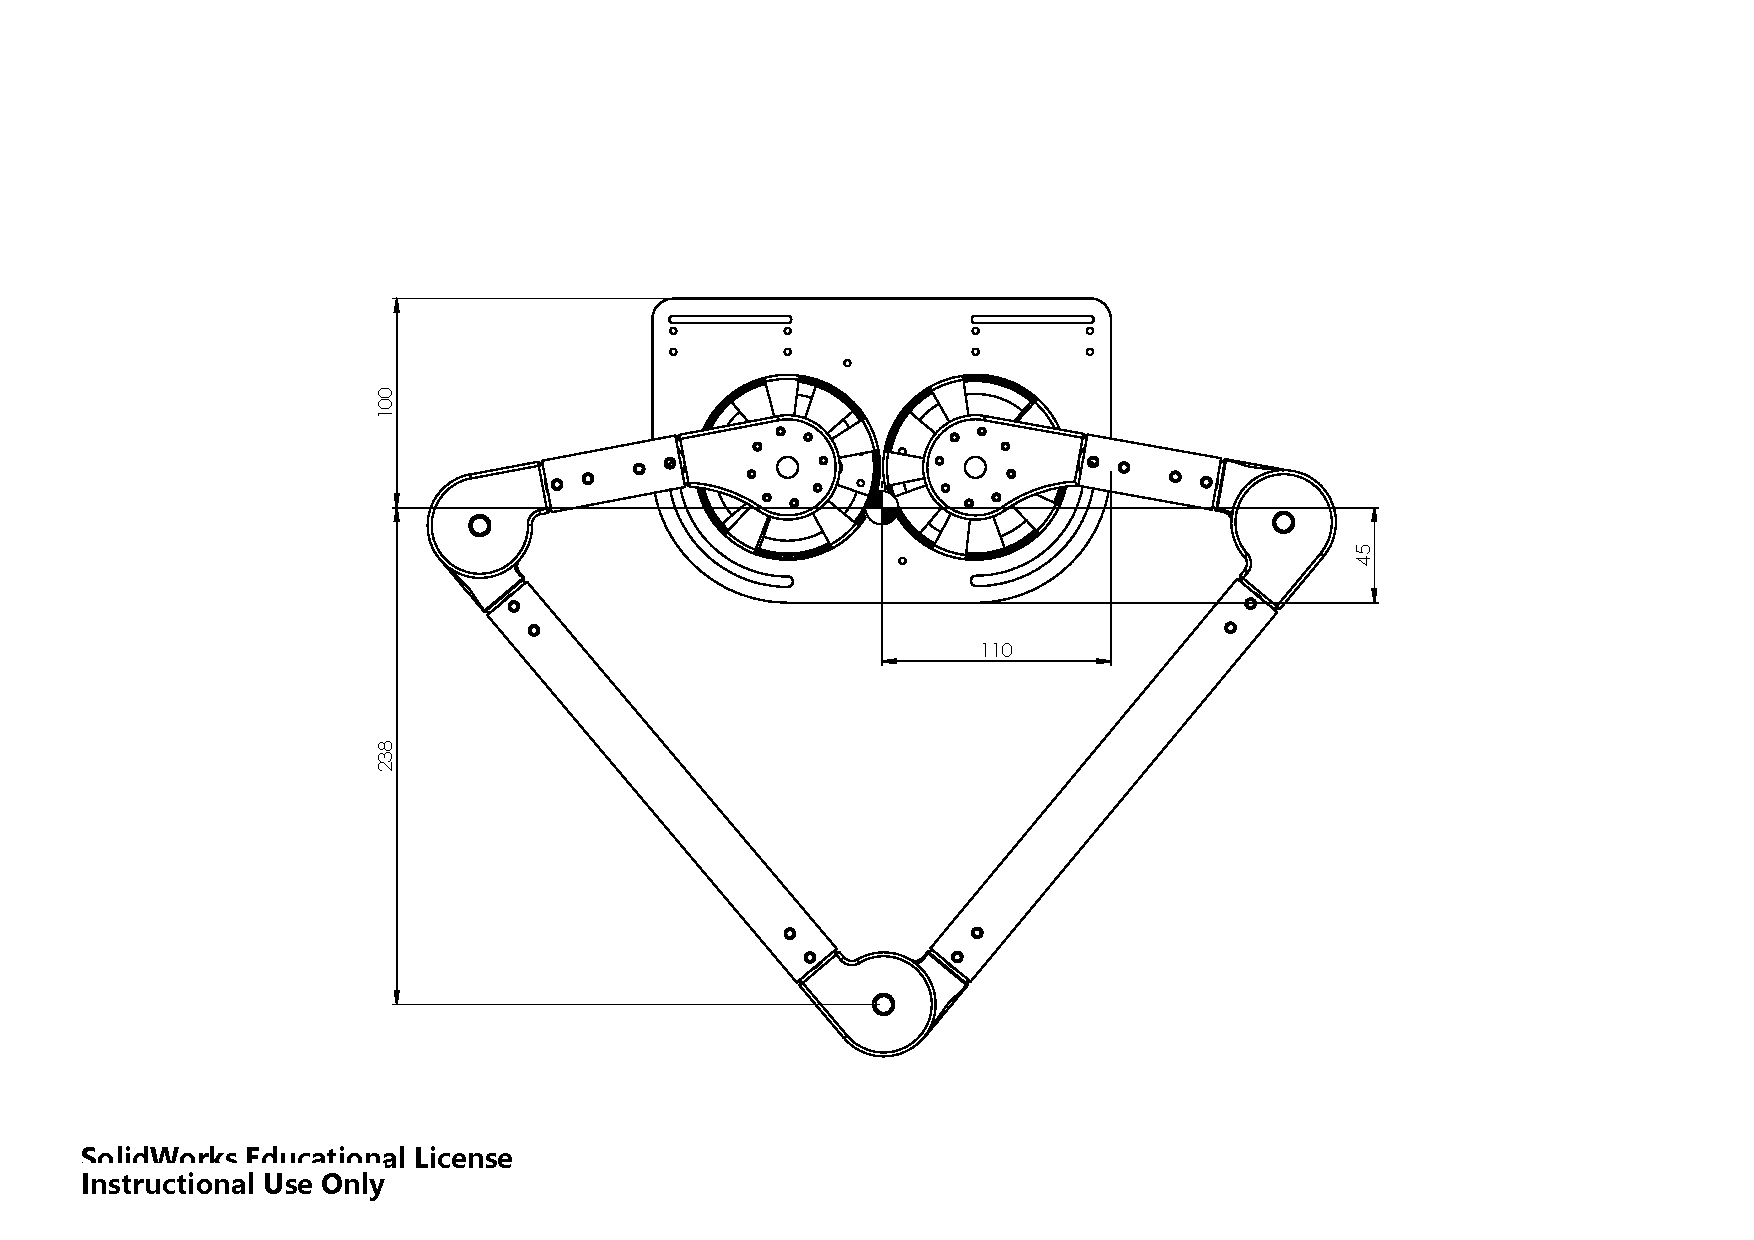
\includegraphics[clip, trim=5cm 2cm 5cm 5cm, page = 1, width=1\textwidth]{images/mechanical/assembly-com.pdf} 
}
\caption{Mass distribution of leg assembly.}
\label{fig:Mass distribution of leg assembly}
\end{figure}

\subsection{Actuator to Body Mass Ratio}
In the study \cite{Kenneally2016} it is stated that as large a proportion of the mass budget as possible should be dedicated to the actuator, in this case the T-Motor U10 Plus BLDC motor. \Cref{tbl:Robot performance comparison} shows that the Baleka robotic leg has the second highest actuator to body mass ratio, second only to the GOAT leg. This performance rating is perhaps biased as the Baleka leg does not have the mass of on-board motor drivers and control.

\section{Mechanical Impedance}
\label{sec:Mechanical Impedance}
\subsection{Linear Guide}

In \cref{sec:Jump Test} a set of jump-tests were performed. By extracting the acceleration data from the video frames of a jump a plot of acceleration vs. time was found as seen in \cref{fig:acc-time-jump}. During the free-fall phase of the jump the mean acceleration was calculated as $-9.51\ m/s^2$. Using this acceleration and the known acceleration due to gravity, the coefficient of kinetic friction for the linear guide, $\mu_k$, can be calculated as in \cref{eq:linear-guide-friction}.  

\begin{equation} \label{eq:linear-guide-friction}
\begin{aligned}
&F_k = F_n \mu_k \\
&\mu_k = \frac{F_k}{F_n} \\
&\mu_k = \frac{|m\ddot{x} - mg|}{|mg|} \\
&\mu_k = \frac{|2.2\times -9.51 - 2.2\times -9.81|}{|2.2\times -9.81|} \\
&\mu_k = 0.031
\end{aligned}
\end{equation}

This value for kinetic friction is minimal and in practise was assumed to have an insignificant effect on jump dynamics. If a more precise mechanical system was developed and jump height control was implemented, then the kinetic friction could be taken into account. In experimentation the jump height was not consistently controllable due to mechanical joint slack.

\subsection{Leg and Joints}

The friction, and to a limited extent the inertial load, of the leg and joints was accounted for during the calibration process for the torque constant $K_t$ in \cref{sec:Motor Model Calculations}. By using force control and the calibration process the joint frictional force that needs to be overcome is indirectly included in the control model.

Due to mechanical joint slack and an imprecise mechanical system, as discussed previously, the inertial and precise frictional load of the leg is difficult to accurately calculate - because of this it is better to experimentally account for all these factors during calibration.

\section{Electronics and Communication}
\subsection{Accelerometer and Gyroscope}

The iNemo board designed and built by Callen Fisher during his masters studies, consisting of a STM32F1 microcontroller with on-board accelerometer, gyroscope and magnetometer, was to be used to measure acceleration data for force measurements and jump phase control. 

Due to time constraints acceleration data was not used or found to be necessary for basic hopping control. Provision was made for mounting the board as close to the center of gravity of the robot as was physically possible, as can be seen in \cref{fig:Final leg design - back} where the final mounting setup is shown. 

The iNemo board was mounted approximately $4\ cm$ from the center of gravity directly over the linear guide. This was achieved by using nylon spacers and the included $3\ mm$ mounting points on the board.

The necessary peripheral configuration and data processing can be easily integrated into the embedded system communication protocol developed in \cref{chap:Software Development} in future. The GitHub page for the iNemo development board can be seen at \url{https://github.com/Callen-Fisher/INEMO-development-board}.

\subsection{Distance Sensor}
A distance sensor was mounted to the base of the mounting plate, as seen in \cref{fig:Final leg design - back}. This provided feedback of the height of the leg's center of mass above the ground.

The leg height was used for height control as well as flight phase determination.

An infra-red distance sensor was chosen with a narrow beam width - this ensures there is minimal reflection off surrounding objects that could interfere with distance readings. The beam reflects off the surface of the ground and a time-of-flight calculation is used to determine distance. Infra-red is open to possible interference from surrounding fluorescent light sources, and this can be accounted for by using it in an area out of direct line of site of light sources. Infra-red was chosen because it is cheaper than an equivalent laser distance sensor.

The Pololu Carrier with Sharp GP2Y0A60SZLF Analog Distance Sensor was used. It requires a $3\ V$ voltage source which can be supplied directly from the micrcontroller which runs off the same voltage. 

The distance sensor outputs an analog signal which is related to the height. This analog signal is fed into the ADC of the microcontroller and using a linear relationship is mapped to the distance. 

The Pololu distance sensor has a range of $10-150\ cm$, which is more than enough for the intended hopping height of $20-50\ cm$ due to the testing rig limits.

The height sensor was calibrated by setting it at $0.1\ m$ from a surface and using a scaling factor to adjust the linear relation between distance and voltage until an accurate measurement was achieved. 

A 3D printed carrier, a render of which can be seen in \cref{fig:distance-sensor-mount}, was designed for the distance sensor which offset the sensor from the mounting plate and placed it in a central location above the linear guide.

\begin{figure}
\centering
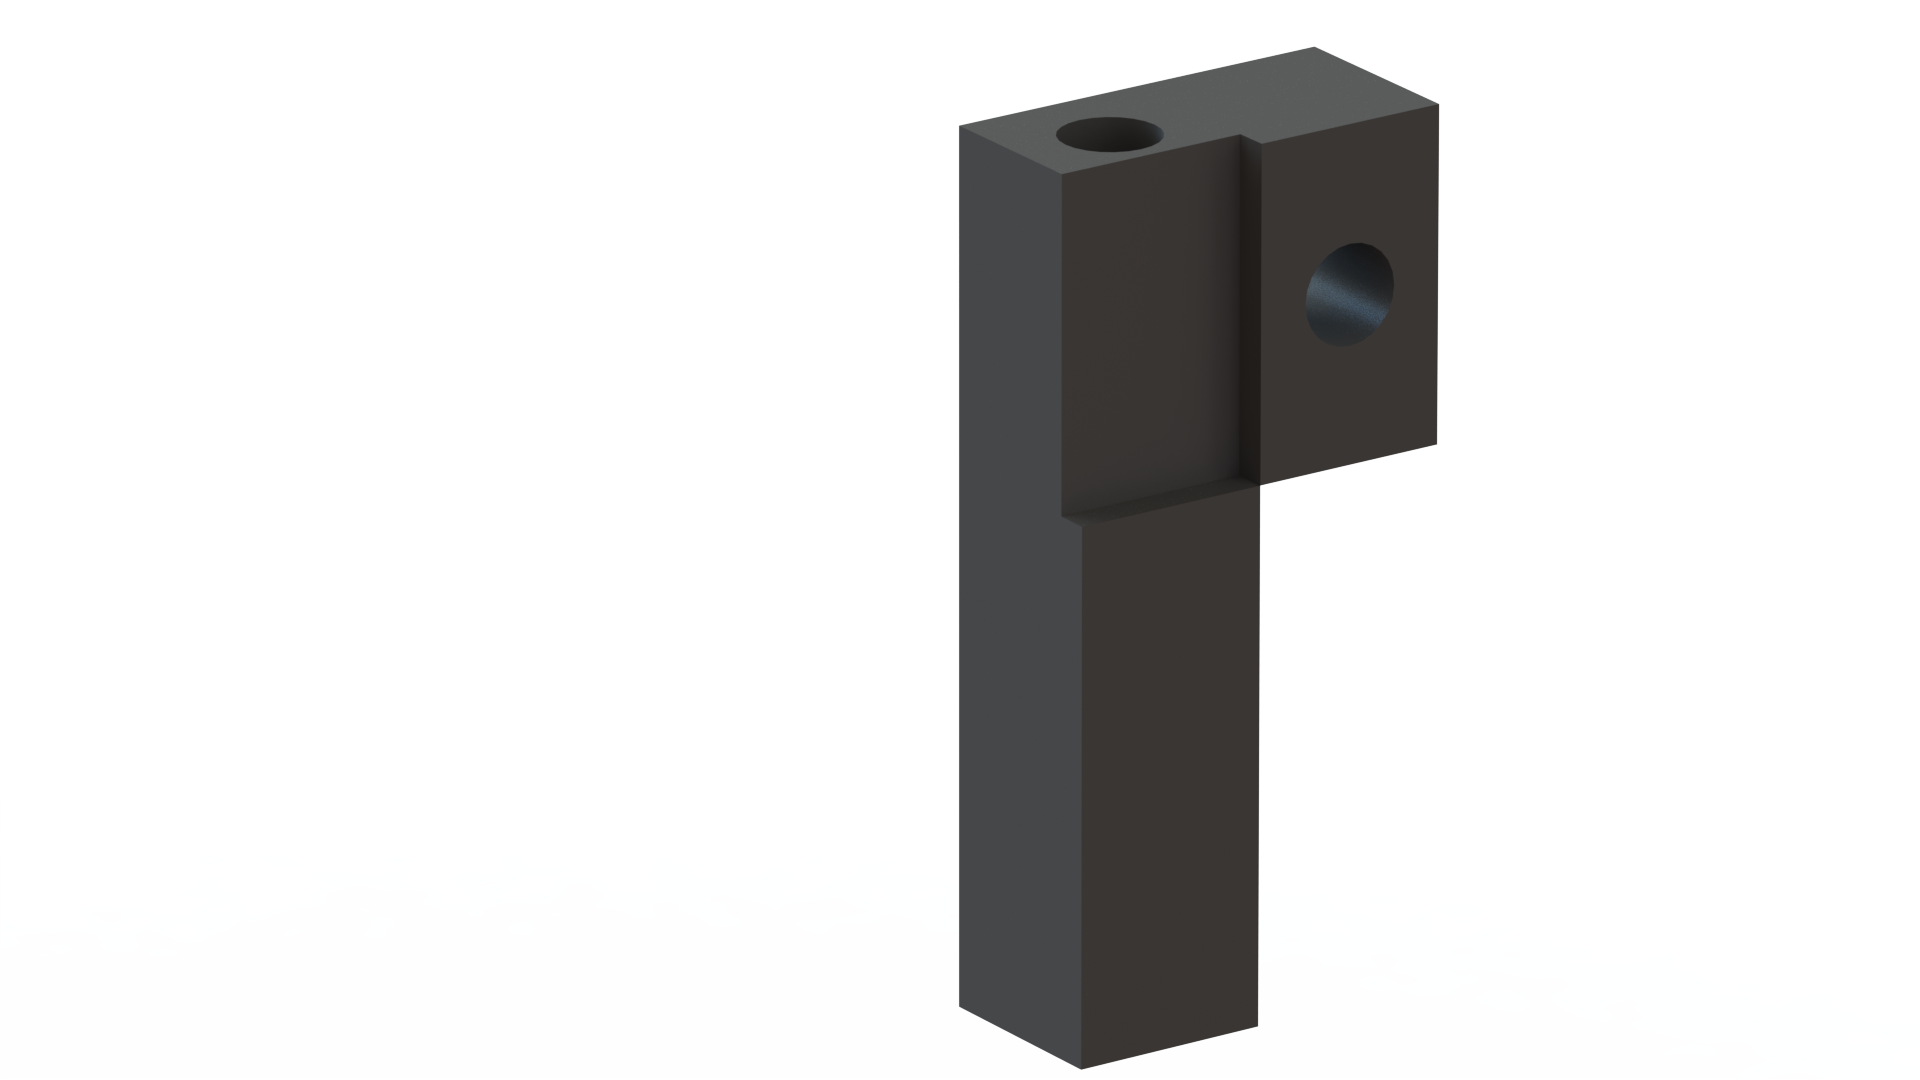
\includegraphics[clip, trim=4cm 0cm 2cm 0cm, width=0.4\textwidth]{images/mechanical/distance-sensor-mount} 
\caption{3D printed PLA distance sensor mount.}
\label{fig:distance-sensor-mount}
\end{figure}

\subsection{Microcontroller}
The microcontroller had to meet the following specifications:
\begin{itemize}
\item 4 x UART Ports
\item 1 x ADC
\item 1 x Floating point unit
\item DMA Capabilities
\item USB Debugging
\item 5V tolerant UART ports
\end{itemize}

Being familiar with the STM32 series of microcontrollers, a STM32F4 board was chosen and met the above specifications with two additional USART ports for future peripheral needs.

\section{Motors and Drivers}

\subsection{Driver Selection}
\label{sec:Driver Selection}

The most important factor when choosing a motor driver for dynamic hopping control is the peak current specification. During the launch phase a current impulse will be used to transfer maximum energy to the flight phase. 

In \cref{fig:motor-current-requirements} the kinematic workspace developed in \cref{sec:Simulation-Kinematics} was combined with a virtual compliance control simulation to determine what the theoretical maximum current requirement would be.

A heat map for motor 1 and motor 2 current draw can be seen, with a maximum current magnitude of $52.3\ A$. This simulation was performed with a nominal virtual spring configuration of: 
\begin{itemize}
\item $K_{s1}=300\ N/m$
\item $K_{s2}=30\ N/m$
\end{itemize}
In order to account for the extra current draw when using damping, $60\ A$ was chosen as the motor driver specification. 

The peak current specification chosen was adequate for the platform in use, but for achieving higher and more fine tuned jump control a higher peak current is needed. This is further investigated in \cref{sec:Jump Test}.

To achieve a controller sampling frequency of $200\ Hz$ a high speed and robust communication protocol is needed. RS-485 was chosen as the preferred protocol for the following reasons:
\begin{enumerate}
\item Robust to noise interference from BLDC motors.
\item Can support high speed data rates up to $1\ MBaud$.
\item Easy to implement and readily available on off-the-shelf microcontrollers.
\end{enumerate}

In practise the motor drivers caused a communication bottle neck due to the time taken for the controllers to respond to control packets sent - ideally the motor driver should be able to receive, process and reply to control packets without a significant delay. This is further investigated in \cref{chap:Software Development}.

The specifications determined above were met by the AMC servo drive and mounting card seen in \cref{fig:AMC Servo Drive and Mounting Card}. 

\begin{figure}
\centering
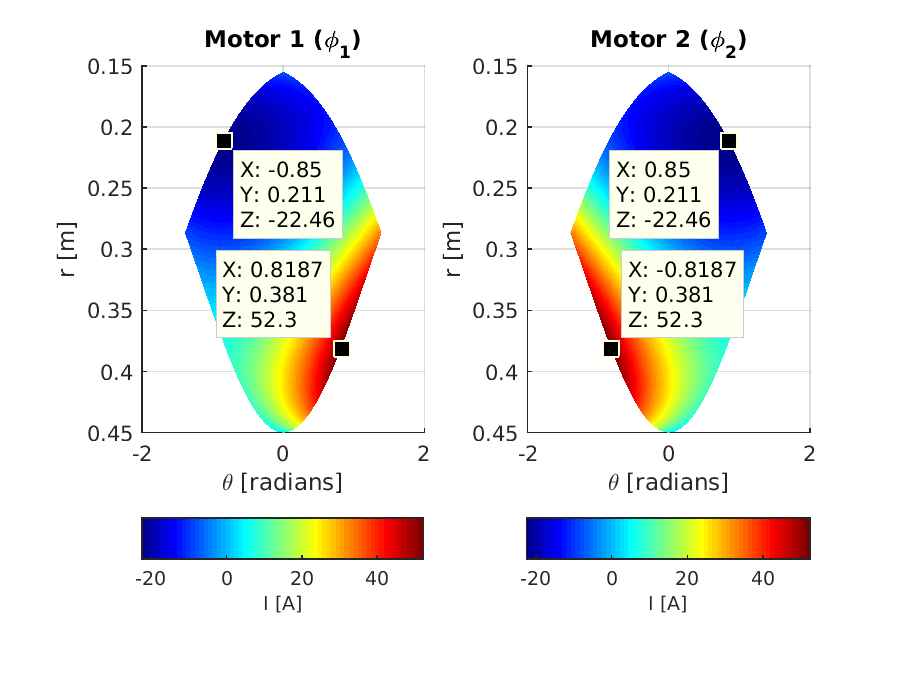
\includegraphics[width=0.8\textwidth]{images/control/forward-kinematic-motor-current.eps} 
\caption{Active compliance motor current requirements.}
\label{fig:motor-current-requirements}
\end{figure}

\begin{figure}
\centering
\subfloat[][AMC DigiFlex Performance Servo Drive.]{
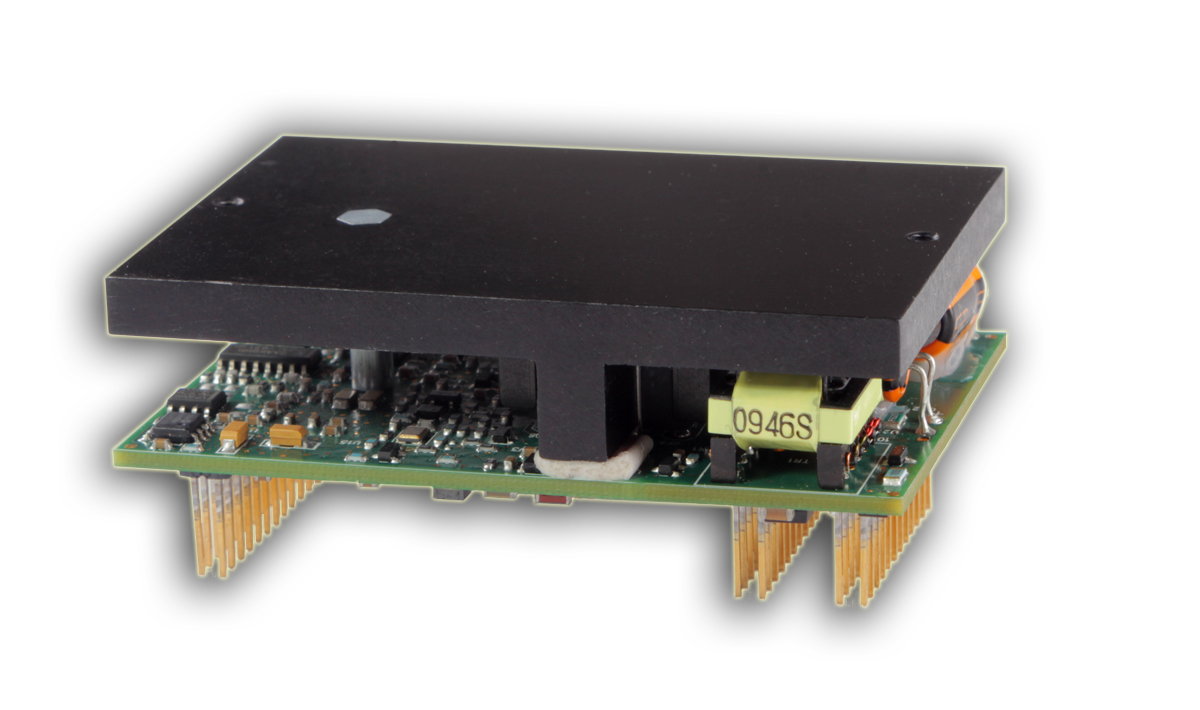
\includegraphics[width=0.3\textwidth]{images/driver/driver.jpg} 
}
\subfloat[][AMC DigiFlex Performance Servo Drive mounting card.]{
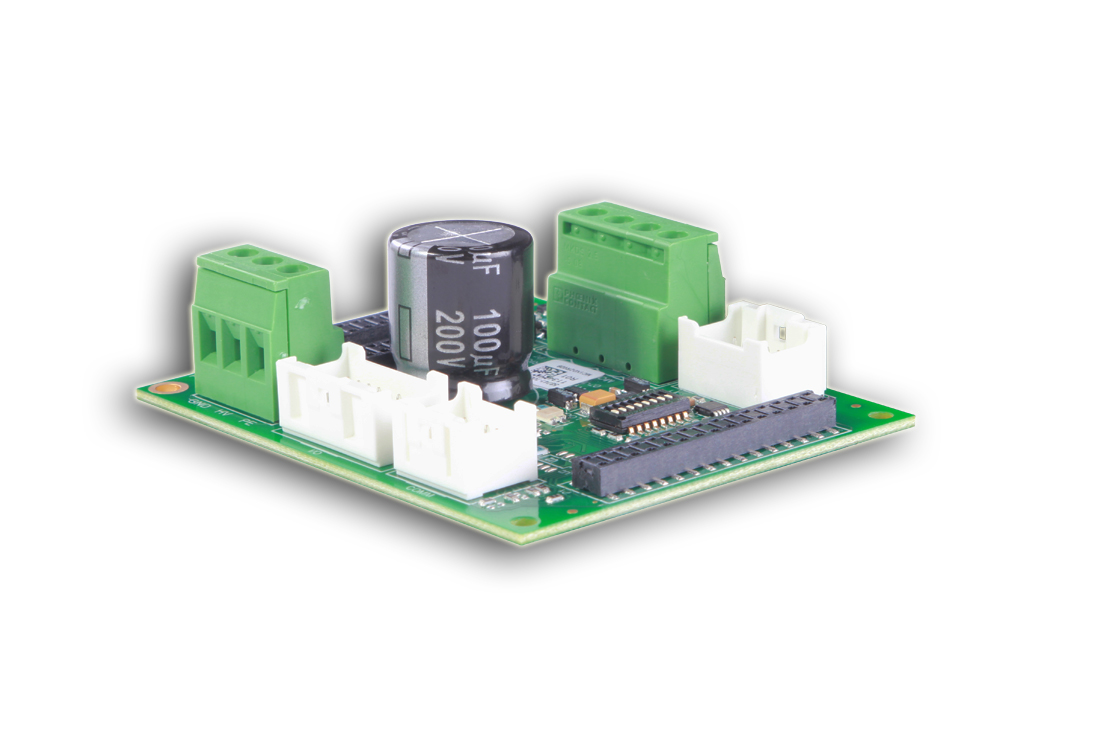
\includegraphics[width=0.3\textwidth]{images/driver/mounting-card.jpg}
} 
\caption{AMC Servo Drive and Mounting Card.}
\label{fig:AMC Servo Drive and Mounting Card}
\end{figure}

\subsection{Motor Selection}
\label{sec:Motor Selection}

A brushless DC motor (BLDC), by definition, has few parts such as brushes that will degrade over time or provide resistance to movement. This is advantageous in robotic systems were repeated high torque operations will be performed.

Due to the recent popularity of BLDC motors in use on quadcopter and other hobby platforms, high performance motors have become more accessible. 

In the case of a direct drive robotic platform, performance is measured by the amount of torque the motor can supply for a given current under load.

In the study by \cite{Kalouche2016} various COTS (commercial off the shelf) motors were compared using the thermal specific torque as a performance measure. The T-Motor U10 Plus was found to have the highest thermal specific torque at $0.42 \frac{Nm}{kgC^o } \text{ at } r_{gap} = 40 mm$ \cite{Kalouche2016}. When compared to the custom made MIT Cheetah motors at $0.71 \frac{Nm}{kgC^o } \text{ at } r_{gap} = 49 mm$ found in \cite{Wang2012} they perform favourably. 

\Cref{fig:Motor performance requirements} visually shows the relationship between torque, current and speed and places the requirements of the Baleka leg on the plot in blue and the specifications of the T-Motor U10 Plus in red. The T-Motor U10 Plus has the following specifications:

\begin{itemize}
\item KV rating: 80
\item Shaft diameter: 15 mm
\item Weight: 500 g
\item No. of Cells (Lipo): 6-14s
\item Max Continuous current(A): 33 A
\item Max Continuous Power(W): 1500 W
\item Internal resistance: $95\ m\Omega$
\end{itemize}

The KV rating of 80 indicates an unloaded speed of $80\ rpm$ per volt. This is on the low end of the scale and generally means the motor can achieve a higher torque at low speed than a higher KV rated motor.

The ideal motor for the robotic platform would achieve high torque, low current draw and a high torque for low speed operation as shown in blue in \cref{fig:Motor performance requirements}. 

The T-Motor U10 Plus sits somewhere in the middle of the performance plot, allowing relatively high speed operation using a 10s battery with adequate torque and current draw specification. Two 5s LiPos in series were used to supply the motors, providing approximately $40\ V$ and a theoretical maximum speed of $3200\ rpm$.

The T-Motor U10 Plus was chosen for the reasons above, as well as the fact that it is a well known and used motor in direct drive robotic projects, being featured in \cite{Duperret} and \cite{Kalouche2016} among others. This is beneficial as they are well documented and it allows us to compare the relative performance between these robotic leg platforms.

\begin{figure}
\centering
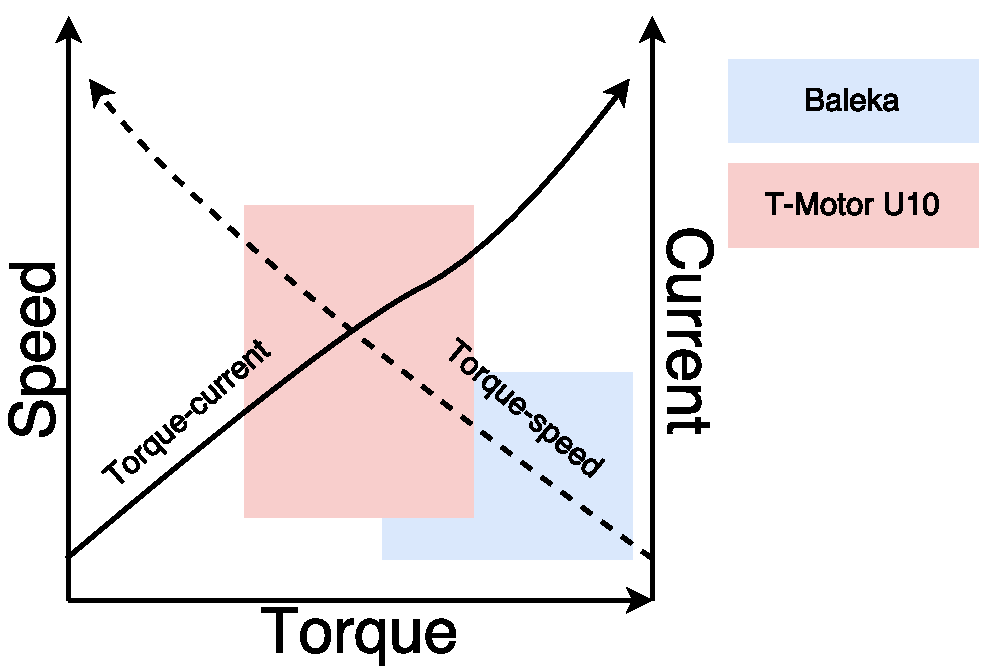
\includegraphics[width=0.6\textwidth]{images/motor/bldc-torque-speed-relation.pdf} 
\caption{Motor performance requirements.}
\label{fig:Motor performance requirements}
\end{figure}

\begin{figure}
\centering
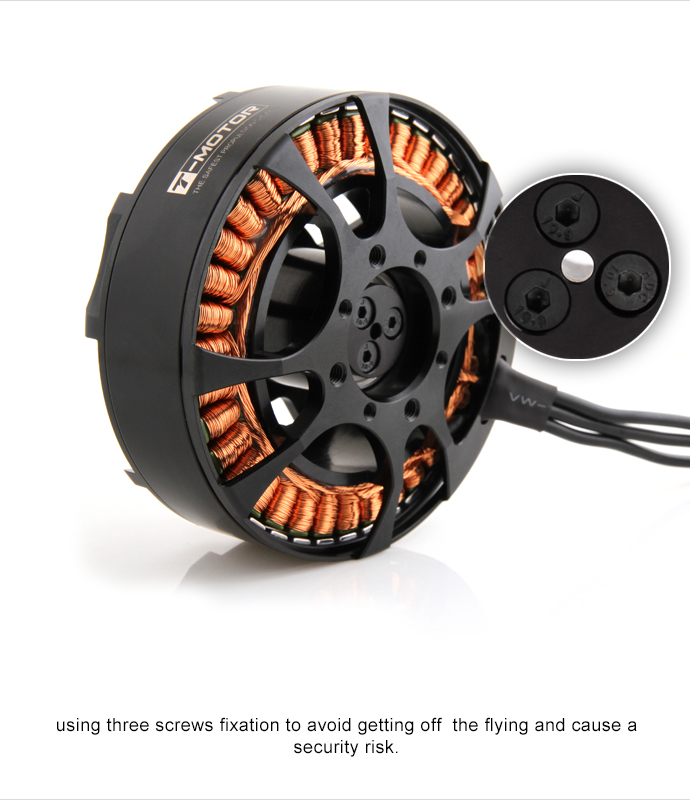
\includegraphics[clip, trim=0cm 5cm 0cm 2cm, width=0.4\textwidth]{images/motor/TMotorU10Plus} 
\caption{T-Motor U10 Plus Brushless DC Motor.}
\label{fig:TMotorU10Plus}
\end{figure}

\subsection{Motor Model Calculations}
\label{sec:Motor Model Calculations}

\subsubsection{Experimental Calculation of $K_t$ and $K_e$}
\label{sec:Experimental Calculation of Kt}

The motor torque constant, $K_t$, was calculated using the torque current relation $\tau = K_tI$. The leg was modelled as a virtual spring-damper system, as seen in \cref{fig:Leg spring-damper virtual model}. 

The spring constant, $K_{s1}$, was set to $200\ [N/m]$, and the damping and torsional spring-damping constants were set to zero. $K_t$ was tuned until the theoretical foot force matched the practical foot force measured via a load cell. The leg was fixed at a set height imposing a radial offset on the virtual spring-damper system.

For a spring constant of $200\ [N/m]$ and a radial offset of $0.15\ m$ a theoretical foot force of $K_{s1}\Delta r = 30\ N$ was expected. A mass of approximately $3\ kg$ was measured with $K_t = 0.08\ [Nm/A]$ set in the virtual leg model controller, resulting in a foot force of $3\ kg \times 9.81\ m/s^2 = 29.43\ [N]$. 

The study in \cite{Kalouche2016}, using the same T-Motor U10 Plus motors, calculated a torque constant of $K_t =  0.072\ [Nm/A]$. This confirms the experimental results obtained above.

For an ideal motor at a constant operating point, $K_e$ will equal $K_t$, as shown in \cref{eqn:ktke}.

\begin{equation} \label{eqn:ktke}
\begin{aligned}
&V_t = K_e\omega_m + IR_m \\
&\tau_m = K_t I \\
&P_{elec.} = V_t I = K_e \omega_m I + I^2 R \\ 
&P_{mech.} = \tau_m \omega_m = K_t I \omega_m \\
&P_{loss.} = I^2 R_m \\
&P_{elec.} = P_{mech.} + P_{loss.} \\
&\therefore K_e\ [V/rad/s]= K_t\ [Nm/A] = 0.08
\end{aligned} 
\end{equation}

Further force calibration and fidelity tests were performed in \cref{sec:Force Control Calibration and Fidelity}.

\subsubsection{Calculation of $R_m$ and $L_m$}
The resistance and inductance of the 3 phase windings of the motor were calculated using a lab multimeter to be $R_m = 47.5\ m\Omega$ and $L_m = 35\ \mu H$ respectively. 

Brushless DC motor windings are usually connected in WYE formation, as seen in \cref{fig:bldc-wye-connection}. This means the measured values for resistance and inductance were line-to-line values and had to be divided by two to get the per phase values above.

\begin{figure}
\centering
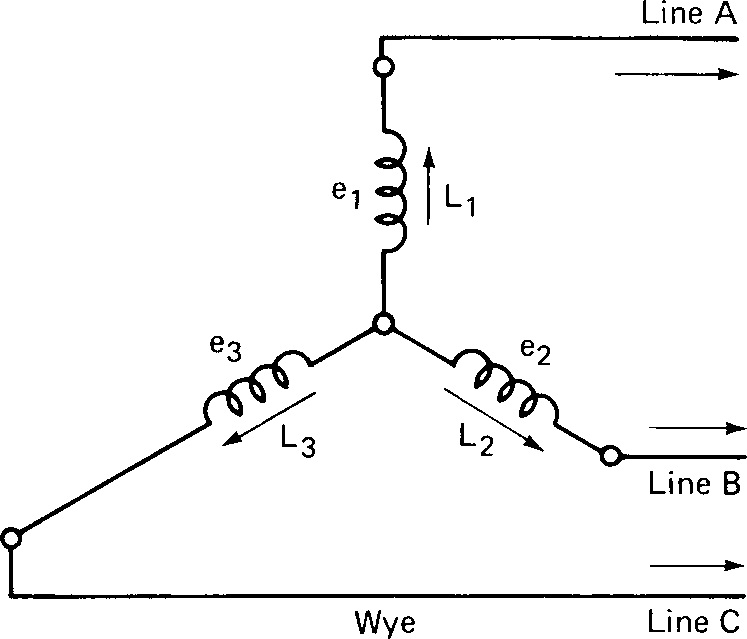
\includegraphics[width=0.4\textwidth]{images/motor/wye.jpg} 
\caption{WYE connected BLDC motor windings.}
\label{fig:bldc-wye-connection}
\end{figure}

\subsubsection{Calculation of $J_m$}
In order to calculate the moment of inertia of the motor, $J_m$, the ratio of acceleration torque to acceleration to steady state needs to be found. By commanding a DC equivalent current input of $1\ A$ and measuring the time taken to reach a steady state velocity, \cref{eqn:Jm} can be used to calculate $J_m$. The velocity vs. time plot used can be seen in \cref{fig:jm-plots}.

\begin{equation} \label{eqn:Jm}
\begin{aligned}
J_m &= \frac{T_{acc.}[N/m]}{a[m/s^2]} \\
&= \frac{IK_t}{a} \\
&= \frac{IK_t}{\frac{\Delta v}{\Delta t}}\ [kg/m^2]
\end{aligned}
\end{equation}

where $I=1\ A$, $K_t=0.08\ Nm/A$, $\Delta v = 1313.906\times \frac{2\pi}{60}\ rad/s$ and $\Delta t = 588.889\times10^{-3}\ s$.

This results in a motor moment of inertia of $J_m = 3.424 \times 10^{-4}\ [kg/m^2]$.

\subsubsection{Calculation of $B_m$}

The motor damping or viscous friction, $B_m$, was assumed to be negligible. Brushless DC motors have near zero damping and will have little effect on the simulated motor model.

\begin{figure}
\centering
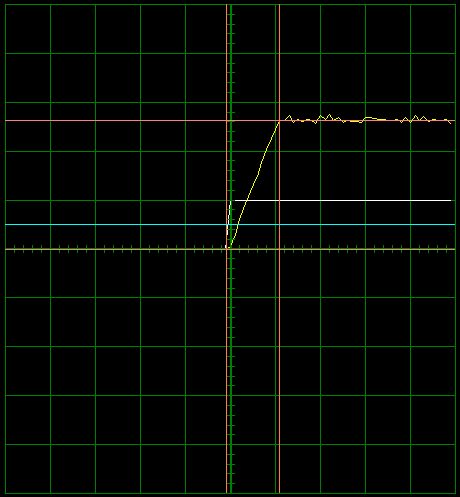
\includegraphics[width=0.5\textwidth]{images/driveware/current-velocity-response} 
\caption{Velocity vs. time plot for 1A equivalent DC command.\\
(500 rpm; 500 ms/div)}
\label{fig:jm-plots}
\end{figure}

\subsubsection{Calculation of $\tau_e$ and $\tau_m$}
The electrical and mechanical time constants of the motor, $\tau_e$ and $\tau_m$ respectively, can be used to plot a root-locus plot with poles at $-\tau_e$ and $-\tau_m$ as can be seen in \cref{fig:ol-motor-rlocus}. This is useful when designing a current controller for the system. $\tau_e$ and $\tau_m$ can be calculated using \cref{eqn:motor-time-constants}.

\begin{equation} \label{eqn:motor-time-constants}
\begin{aligned}
&K_m = \frac{1}{B_m} \\
&\tau_m = \frac{J_m}{B_m} \\
&K_e = \frac{1}{R_m} \\
&\tau_e = \frac{L_m}{R_m} 
\end{aligned}
\end{equation}

From \cref{eqn:motor-time-constants} and using the previously calculated motor constants, $\tau_e = 7.368 \times 10^{-4}$ and $\tau_m = 3.424 \times 10^{-4}$. This is assuming the motor viscous friction $B_m$ is insignificant which is usually the case in mechanically well made BLDC motors.

The resulting motor model open loop root-locus plot can be seen in \cref{fig:ol-motor-rlocus}. As expected the system has only negative real roots and will be stable in open loop.

\begin{figure}
\centering
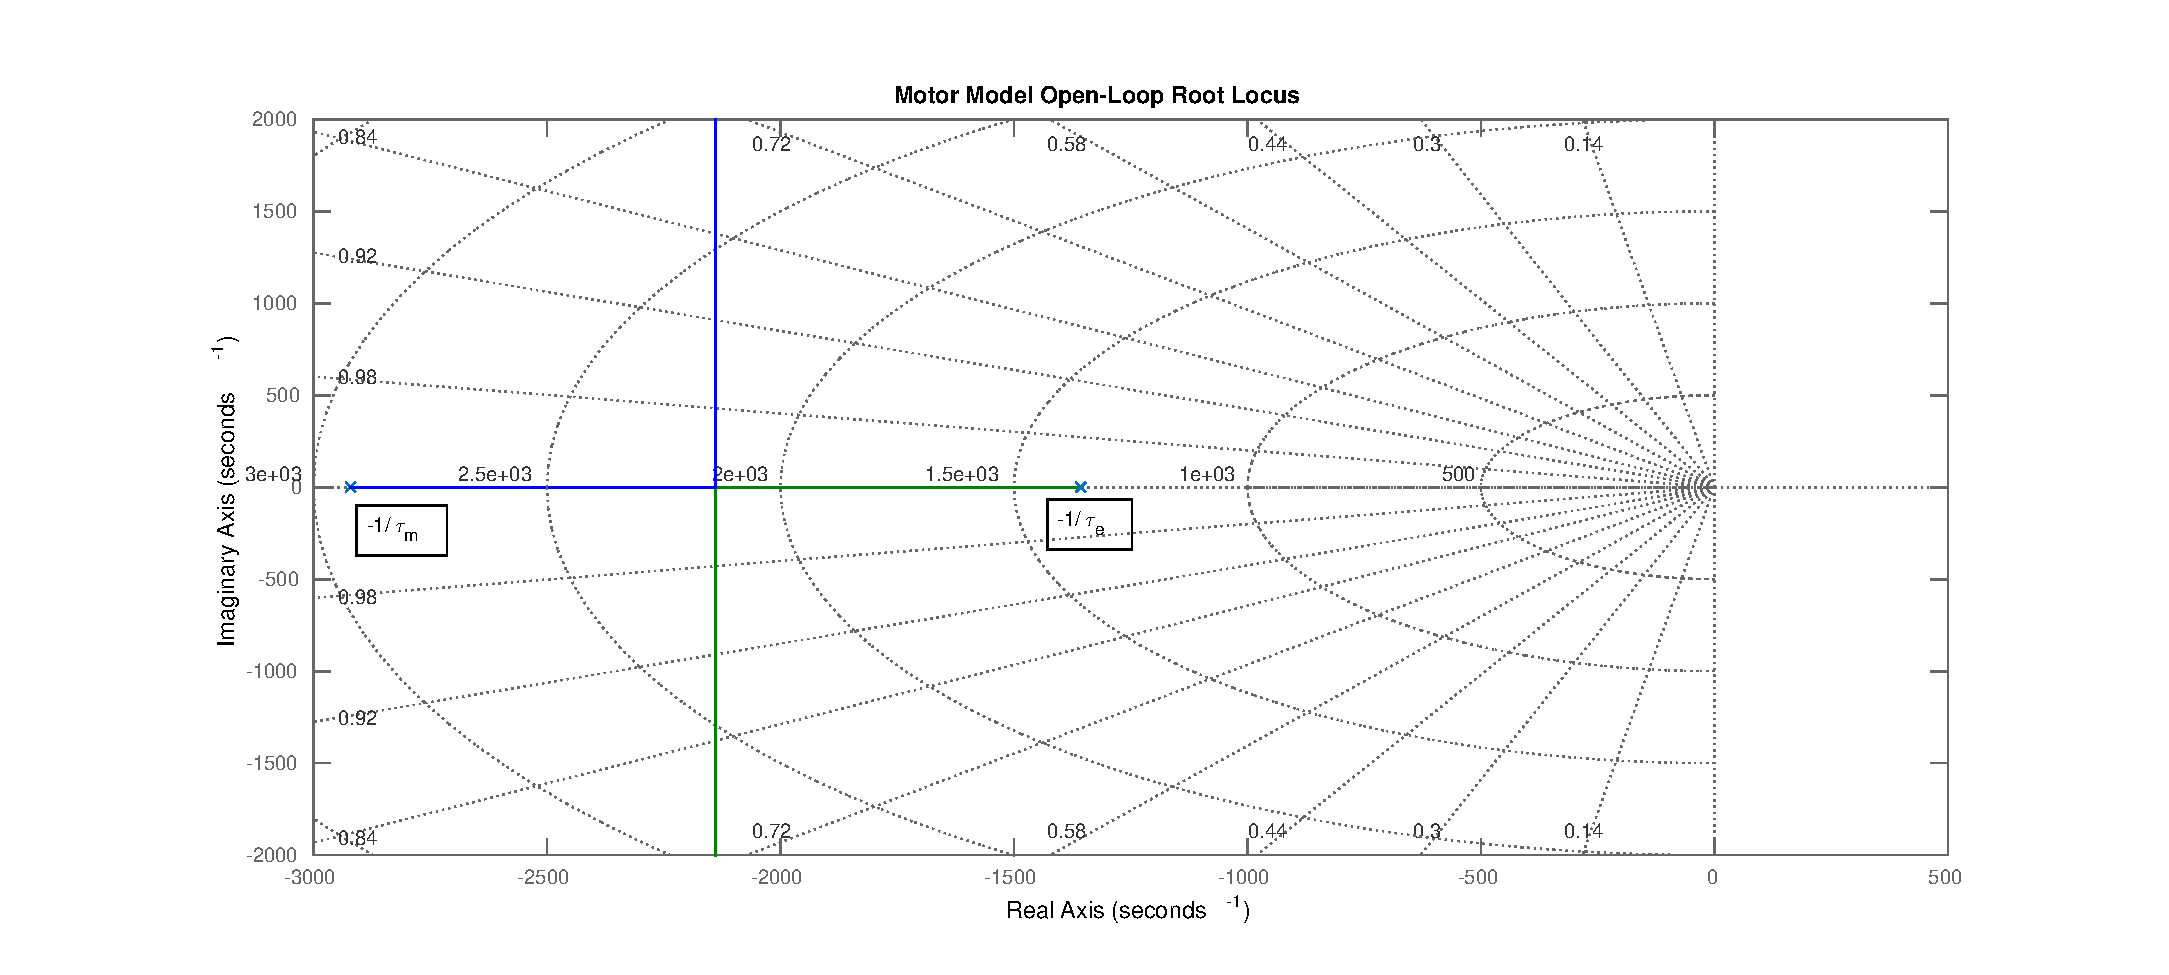
\includegraphics[width=1\textwidth]{images/motor/ol-motor-rlocus} 
\caption{Motor model open loop root-locus plot.}
\label{fig:ol-motor-rlocus}
\end{figure}


\subsection{Driver Configuration}
\label{sec:Driver Configuration}

The AMC drivers allow extensive customisation. After the motor, encoder, and general communication control parameters are configured, the PID control loops of the drivers can be configured, as seen in \cref{fig:AMCControlLoops}.

The motor drivers were initially configured with both on-board PID current and position control loops enabled. This allowed initial modelling of the motors, configuring of the motor encoders, and determining of the position limits (in counts). For control of the leg, the position control loop was finally implemented on the STM32F4 microcontroller, while using the existing current control loop of the motor drivers. The custom position control loop was indirectly implemented using the spring-damper virtual model and force control by setting the polar coordinate set-points, in comparison to the AMC driver position loop which used a PID controller specifically controlling position.

The AMC drivers were configured using the AMC Driveware configuration software, which provided an oscilloscope to measure the relevant motor responses as seen in \cref{fig:jm-plots,,fig:current-tuning-plots,,fig:position-tuning-plots}.

\begin{figure}
\centering
\includegraphics[clip, trim=2cm 5cm 2cm 8cm, page = 114, width=1\textwidth]{pdfs/AMC_DriveWareSoftwareManual.pdf} 
\caption{AMC DigiFlex Performance Servo Drive control loops (AMC, 2014).}
\label{fig:AMCControlLoops}
\end{figure}

\subsubsection{Current Control Loop}

By using a 1 A 120Hz square wave current command the current PI control loop was tuned, as seen in \cref{fig:current-tuning-plots}. Initially both  the proportional gain, $K_p$, and the integral gain, $K_i$, were set to zero. $K_p$ was slowly increased until the final amplitude of the current output just started to overshoot. $K_i$ was then set to minimize the steady state error. 

Values of $K_p = 0.277$ and $K_i = 0.262$ were obtained. Both motors were found to operate optimally with the same PI gain values.

\begin{figure}
\centering
\subfloat[][Motor driver current loop pre-tuning.\\ 
(200 mA; 5 ms/div)]{
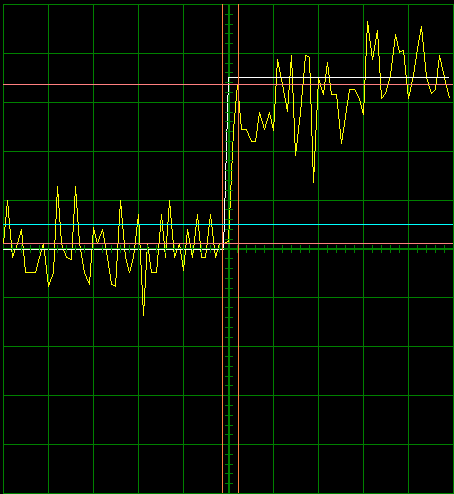
\includegraphics[width=0.4\textwidth]{images/driveware/current-pre-tuning-plot.png} 
}
\subfloat[][Motor driver current loop tuning - 1A 120Hz square wave command.\\(1 A; 1 ms/div)]{
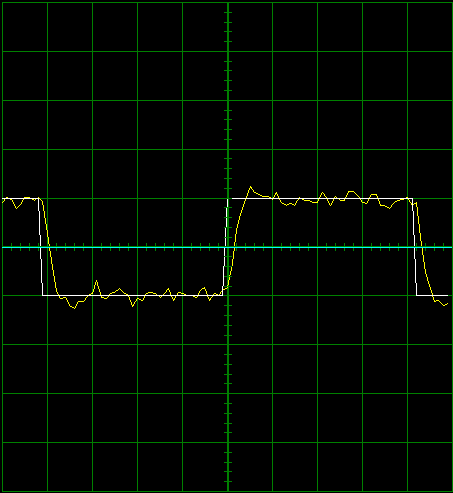
\includegraphics[width=0.4\textwidth]{images/driveware/current-tuning-plot.png} 
}
\caption{Motor driver current loop tuning plots.}
\label{fig:current-tuning-plots}
\end{figure}

\subsubsection{Position Control Loop}
The on-board AMC motor driver control loop was set up to test the encoder configuration. The encoder and relevant position limits can be seen in \cref{sec:motor-encoders}. 

A 1Hz sinusoid was used to tune the PID control loop gains. Values of $K_p = 0.0005793$, $K_i = 0.0006052$ and $K_d = 2.769e^{-9}$ were found to achieve optimal set-point tracking as seen in \cref{fig:position-tuning-plots}. The sinusoidal set-point can be seen in white and the position feedback in yellow. A 10-30 ms lag time can be seen due to the inertial load. This lag time causes a dead-band which should be considered when implementing a controller. 

These tests were performed with the leg attached - the inertial load provided by the leg made PID control loop tuning possible, whereas without any inertial load the BLDC motors overshot their set-point.

\begin{figure}
\centering
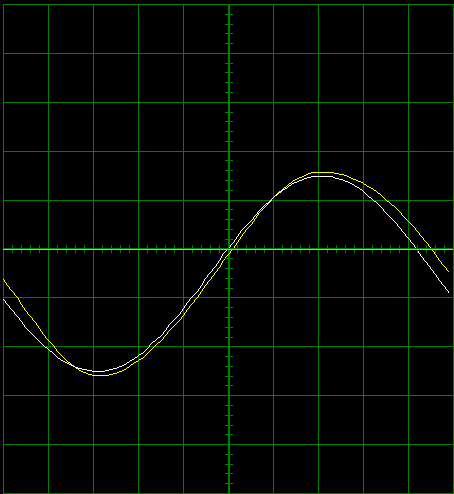
\includegraphics[width=0.4\textwidth]{images/driveware/position-tuning-plot} 
\caption{Motor driver position loop tuning - (-350:200) count 1Hz sinusoid command with 300 count offset.\\(100 ct; 100 ms/div)}
\label{fig:position-tuning-plots}
\end{figure}

\subsection{Motor Encoders}
\label{sec:motor-encoders}

The Avago Technologies HEDL-5640-A13 rotary encoder was used for feedback of encoder position to the motor drivers which then calculate the motor position and velocity relative to a starting encoder count position. 

The encoder has the following specifications:
\begin{itemize}
\item Optical sensing.
\item Incremental counting.
\item 500 counts per revolution.
\end{itemize}

The Avago encoder was chosen for its light, easily mountable frame along with the relatively high resolution position feedback of $0.72 deg./count$.
 
A shaft was designed to mount to the rear of the BLDC motor and interface to the encoder. The shaft was designed in OpenSCAD using programmatic CAD and can be seen in \cref{fig:encoder-shaft}. It was 3D printed by Justin Pead in White Lab using PLA plastic. 

The shaft was designed to be mounted using three hex screws to the provided mounting point on the rear of the motors. A star configuration was used for the interface between the shaft mounting point and the cylindrical encoder shaft so that these hex screws could be accessed easily.

Ideally the shaft should be milled using metal for better heat dissipation. Initially, before the aluminium mounting plate was used, the encoder shafts warped slightly while in operation and had to be bent back into shape. 3D printing was used for rapid prototyping and due to cost considerations.

\begin{figure}
\centering
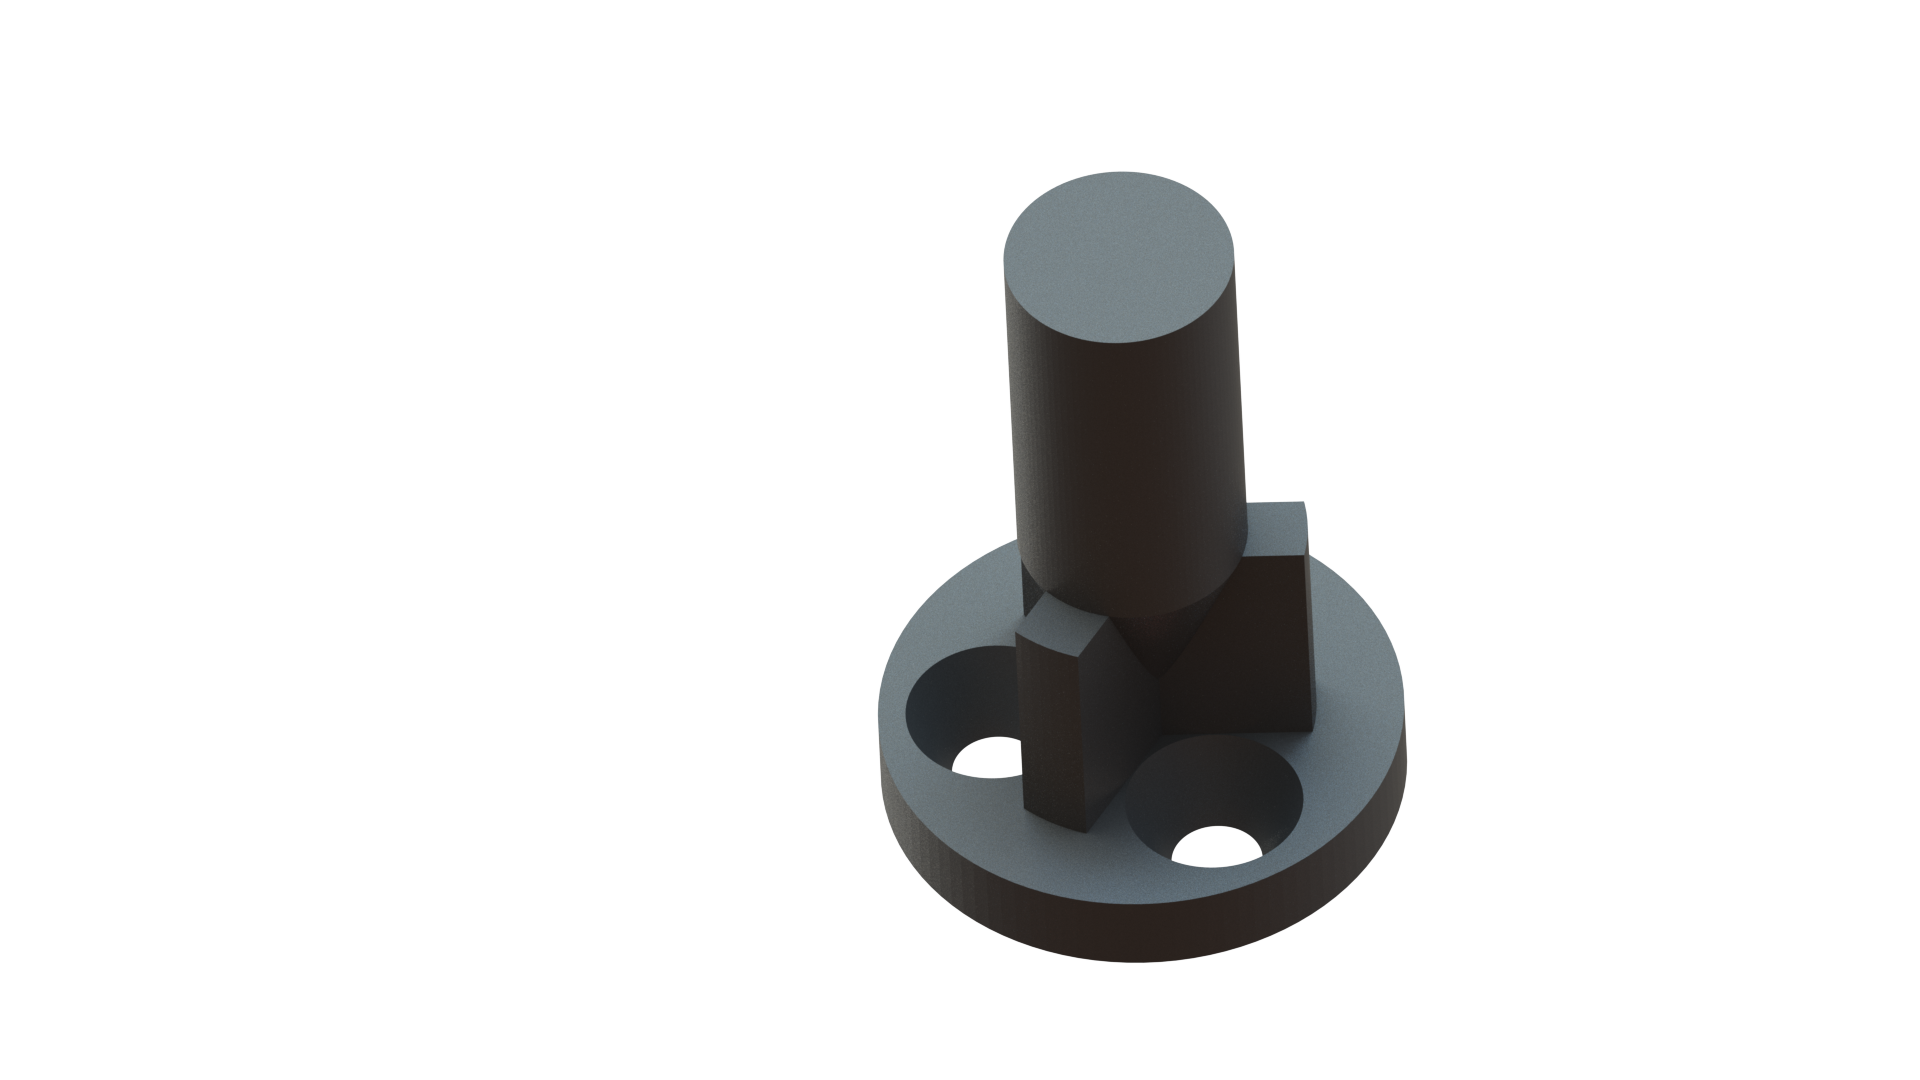
\includegraphics[clip, trim = 6cm 1cm 3cm 1cm, width=0.3\textwidth]{images/mechanical/encoder-shaft} 
\caption{3D printed PLA motor encoder shaft.}
\label{fig:encoder-shaft}
\end{figure} 
